%!TEX root = ../thesis.tex
\chapter{Quad-tree mesh in 2D analysis}

\section{Introduction}
\paragraph{}
The main objective of this chapter is to introduce a way that can utilize the engineering design available in CAD or other popular commercial softwares for 2D case.
The data format that used in almost all engineering design softwares that can represent the geometry exactly is IGES file.
It will be used as a bridge between design and numerical analysis.

\paragraph{}
After the NURBS represented exact geometry has been extracted from the IGES file, a quad-tree mesh generation algorithm described in \ref{qt_sc:quadtree} will be adopted to generate high quality mesh.
Either the NURBS basis functions or the traditional shape function can be used as the shape function of the SBFEM solver.
% We further extend the method to problems with singularities within the framework of linear elastic fracture mechanics.
The proposed method enhances the conventional SBFEM and the salient features of the method are:
    \begin{itemize}
        \item No human effort need to generate the mesh
        \item Exact geometry will be retain
        \item High quality mesh from the quad-tree algorithm
    \end{itemize}
\paragraph{}
This chapter is organized as follows.
The CAD output (iges files) will be introduced first.
After that, an overview of the algorithm that can generate quadtree mesh will be provided.
The accuracy and the convergence properties of the proposed techniques are demonstrated with benchmark problems in the context of linear elasticity, followed by concluding remarks in the last section.
\pagebreak

\section{CAD output in 2D}
\label{qt_sc:iges}
\paragraph{}
IGES\cite{IGES1983} files are used as the bridge between engineering design and numerical analysis.
As a standard file format in engineering design industry, it is supported by almost all design softwares all over the world.
Consequently, by utilizing it we are able to minimize the human effort on mesh generation.

\subsection{Parse geometry in IGES file}
\paragraph{}
The IGES file (explained in detail in \ref{lr_sc:iges}) provides all information that describe the input geometry.
Abstract structure of the IGES file that describe a 2D geometry can be regarded as a simple curve-surface structure.
In other words, it defines the input geometry as certain number of surfaces with different colors.
Different colors represented different material properties in engineering practice.
Each surface contains a list of curve index which is corresponding to the curve information described in IGES file.

\paragraph{}
When IGES file is feed into the programme, each line in the directory entry will be parsed entity by entity.
Parameter in directory entry describe the type and reference to other useful values for the entity.
An entity may reference to one or many entities in directory entry.
Detail of the specification of each entity is explained in \cite{Nasr2007} in detail.

%=====================================================================================================================%
\subsection{Output to mesh generator}
\paragraph{}
The output file that the mesh generator read in will be a shorter summary of the input geometry.
Boundary representation will be kept as the data structure to describe the input geometry.
However, some fields apart from curve and surface will be added.
In the output file, geometry description will be organized as key points, polylines and surfaces.
The key points define the coordinate of all points and polylines are used to represented all curves including NURBS curves for simplification.
NURBS curves can be used directly by the mesh generator as well in \ref{qt_sc:nurbs} but it is found the computational cost in calculation of distance between points to NURBS curves surpass the merits of using it directly.
The exact geometry can be retained by projected the nodes on the boundary back to the origin NURBS curves at the end.

\paragraph{}
Represent a straight line with polyline will not be a problem, first and the last points will be enough to exact representation.
However, that is not the case for curves where curvature is not always zero.
Although using more points must increase the quality of polyline representation, computational cost in the mesh generation when calculating the distance increases at the same time.
Yet, selecting few points that result in a bad polyline representation leads to a poor quality mesh.
Elements may be twisted after the nodes on the boundary are projected to the origin curves.
As a consequence, a quantified index that can control the number and the position of the vertices on the polyline is necessary.

%=====================================================================================================================%
\subsection{Discretization of circular arc}
\paragraph{}
Chord ratio can be a good indicator for circular arc.
The arc length to chord length ratio $\frac{a}{L}$ illustrated in fig.~\ref{qt_fig:iges_chord_ratio} can be expressed in angle $\alpha$ as:
    \begin{equation}
        \frac{a}{L} = \frac{
            \sqrt{2-2\cos\alpha}
        }{\alpha}
        = \frac{
            2\sin\frac{\alpha}{2}
        }{\alpha}
    \end{equation}

The maximum angle $\alpha$ satisfy arc length to chord length ratio $\frac{a}{L} > 1-\epsilon$ with $
    \sin\frac{\alpha}{2} = 1 - \frac{x^3}{6} + O(x^7)
$ can be derived as:
    \begin{equation}
        \alpha < \sqrt{24 \epsilon}
    \end{equation}

    \begin{figure}[h!]
        \centering
        \scalebox{1.2}{
            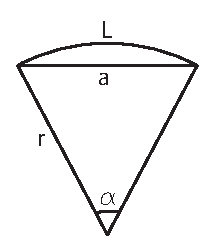
\includegraphics{quadtree/images/iges_chord_ratio.eps}
        }
        \caption{Chord length for circular arc}
        \label{qt_fig:iges_chord_ratio}
    \end{figure}

%=====================================================================================================================%
\subsection{Discretization of NURBS curves}
\paragraph{}
For NURBS curve there is no closed form chord ratio that can be utilized.
However, similar idea can be applied numerically.
The NURBS curves are first divided into serval smaller ones based on the knot vector.  % may be explained in detail
Since the order of each sub-divided NURBS curve used in engineering softwares are predominantly lower or equal to three, the sub-curves then can be divided into two classes, convex curves or concave curve with an inflection point as shown in fig.~\ref{qt_fig:iges_chord_ratio_nurbs}.
    \begin{figure}
        \begin{subfigure}[b]{0.5\linewidth}
            \centering
            \scalebox{0.5}{
                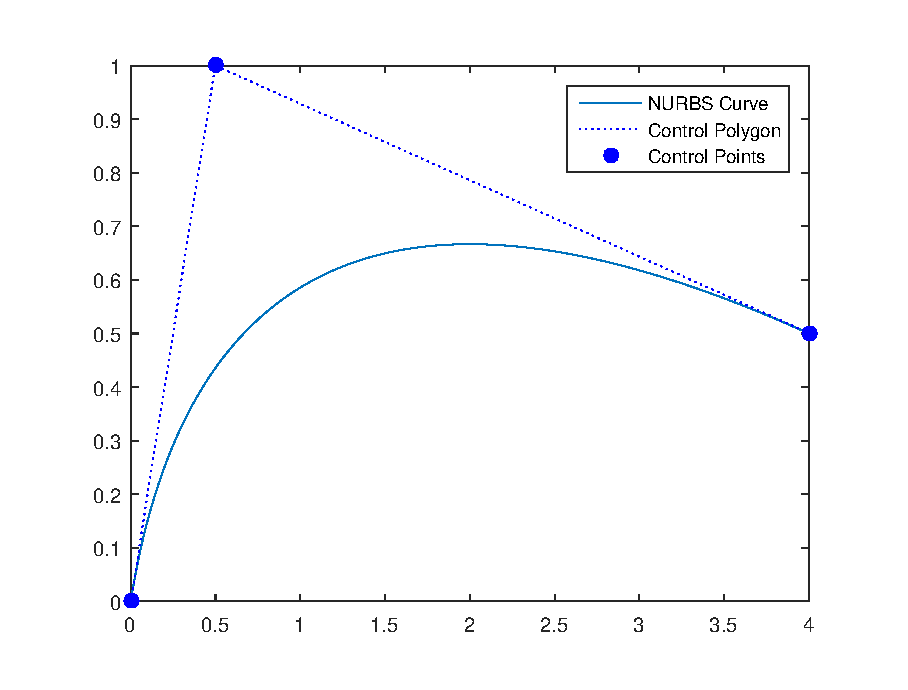
\includegraphics{quadtree/images/iges_chord_ratio_nurbs_convex.eps}
            }
            \caption{Convex}
        \end{subfigure}
        \begin{subfigure}[b]{0.5\linewidth}
            \centering
            \scalebox{0.5}{
                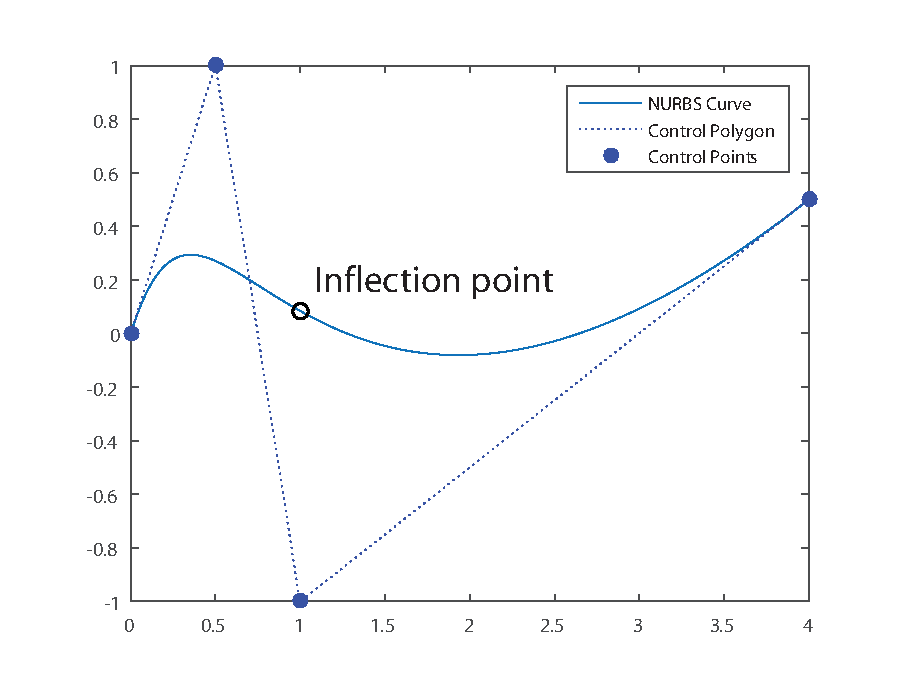
\includegraphics{quadtree/images/iges_chord_ratio_nurbs_concave.eps}
            }
            \caption{Concave with an inflection point}
        \end{subfigure}
    \caption{Type of sub-devided NURBS curves: convex and concave with an inflection point}
    \label{qt_fig:iges_chord_ratio_nurbs}
    \end{figure}

In order to determine the target NURBS curve is convex or concave, a cross product to assess whether the control net will be conducted.
Assuming the target sub-divided NURBS curve is cubic, there will be four control points $P_1,P_2,P_3$ and $P_4$.
If signs of $cross(\overrightarrow{P_1P_2},\overrightarrow{P_2P_3})$ and $cross(\overrightarrow{P_1P_2},\overrightarrow{P_2P_3})$ are the same, then the curve is convex. Otherwise it will be concave.

%=====================================================================================================================%
\subsubsection{Convex curves}
\label{qt_ssc:convex_curves}
\paragraph{}
Start with the simple case, in the situation illustrated in fig.~\ref{qt_fig:iges_chord_split_convex_sum} where line $C(u_0)C(u_n)$ and the NURBS curve form a convex set, we are looking for a point $C(u_m)$ on the curve so that $C'(u_m)$ is parallel to $\overrightarrow{C(u_0)C(u_n)}$
    \begin{figure}[h!]
        \centering
        \scalebox{0.8}{
            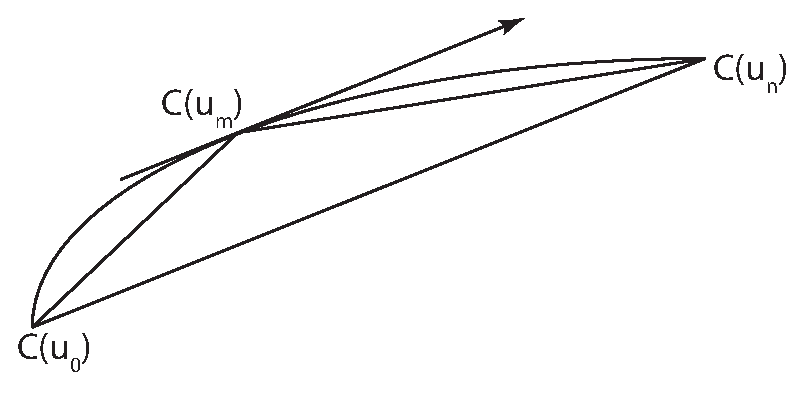
\includegraphics{quadtree/images/iges_chord_split_convex_sum.eps}
        }
        \caption{Discretization for convex NURBS curve}
        \label{qt_fig:iges_chord_split_convex_sum}
    \end{figure}

The target is then split one NURBS curve segment into two.
If any arc length to chord length ratio of these two ratio is below the tolerance given, the splitting will be processed recursively.
Based on the properties of the convex set, there is one and only one parameter $u_m$ that satisfy the condition.
As a consequence, numerical method such as Newton's method can be adopted to find it.
For a given $u_n$, the next iteration will be:
    \begin{equation}
        u_{n_{new}} =  u_n - \frac{f(u_n)}{f'(u_n)}
    \end{equation}

where 
    \begin{equation}
        f(u) = C'(u) \begin{bmatrix}
            - C_y(u_n) + C_y(u_0) \\
            C_x(u_n) - C_x(u_0)
        \end{bmatrix}
    \end{equation}


%=====================================================================================================================%
\subsubsection{Concave curves}
\paragraph{}
As can be seen in fig.~\ref{qt_fig:iges_chord_ratio_nurbs}, the extracted cubic NURBS curve will have no more than one inflection point.
The reason for that is because the target function is cubic and hence the second derivative of it will be in first order.
Consequently, numerical method such as Newton's method can be used to find this unique point.
After that, the curve can be divided into two convex ones and algorithms introduced in \ref{qt_ssc:convex_curves} can be used separately.
The Newton's iteration can be written as
    \begin{equation}
        u_{n_{new}} = u_n - \frac{f(u_n)}{f'(u_n)}
    \end{equation}

where
    \begin{equation}
        f(u) = C''(u)
    \end{equation}

%=====================================================================================================================%
\subsubsection{Calculation of the arc length}
\paragraph{}
The arc length of the NURBS curve defined on $u \in [u_0, u_1]$ can be expressed as
    \begin{equation}
        L = \int_{u_0} ^{u_1} \sqrt{C_x^2(u) + C_y^2(u)} du
    \end{equation}

The integration can be solved by the help of the numerical integration quadrature described in \ref{iso_subsection:numerical_integration} as:
    \begin{equation}
        L = \sum_{i=0}^n a_i \sqrt{C_x^2(u_i) + C_y^2(u_i)}
    \end{equation}

% \begin{algorithm}
% \caption{Discretization of a nurbs curve}
% \begin{algorithmic}[1]
%     \Procedure{YourFunction}{$x$}
%     \State Do Something
%     \EndProcedure
% \end{algorithmic}
% \end{algorithm}

\section{Quad-tree structure}
\label{qt_sc:quadtree}
\paragraph{}
After the geometry information is exported from the IGES file, it can be feed into the quad-tree algorithm to generate mesh of the problem domain.
As an algorithm based on computational geometry, it require great amount of numerical operation and hence the result may be sensitive to the tolerance.
An absolute tolerance may not be able to handle problem with very large or small geometric size.
As a consequence, the first step is to normalize the geometry into a uniform space ($10\times10$ is used in this chapter).

\subsection{Background mesh}
\paragraph{}
Background mesh describes a mesh in the background. %fig
Its density is decided by the geometry.
This section will introduce the procedure to generate the background mesh.
\paragraph{}
First of all, we start with one square which is the root of the tree.
The size of it will be slightly larger than the normalized input geometry and it is selected as $16 \times 16$ in this chapter.
After that, the root square will be divided into millions (defined by resolution, defined as $2^{res} \times 2^{res}$) smaller ones like pixels in the image.
Then, $2^{s_{max}} \times 2^{s_{max}}$ ``pixels'' will be group into the first layer of the tree, or initial background mesh as shown in fig.~\ref{qdt_fig:qdt_initial_mesh}.
It is used to control the maximum allowable mesh size globally or separately for different material regions.

\begin{figure}[!ht]
    \centering
    \scalebox{0.8}{
        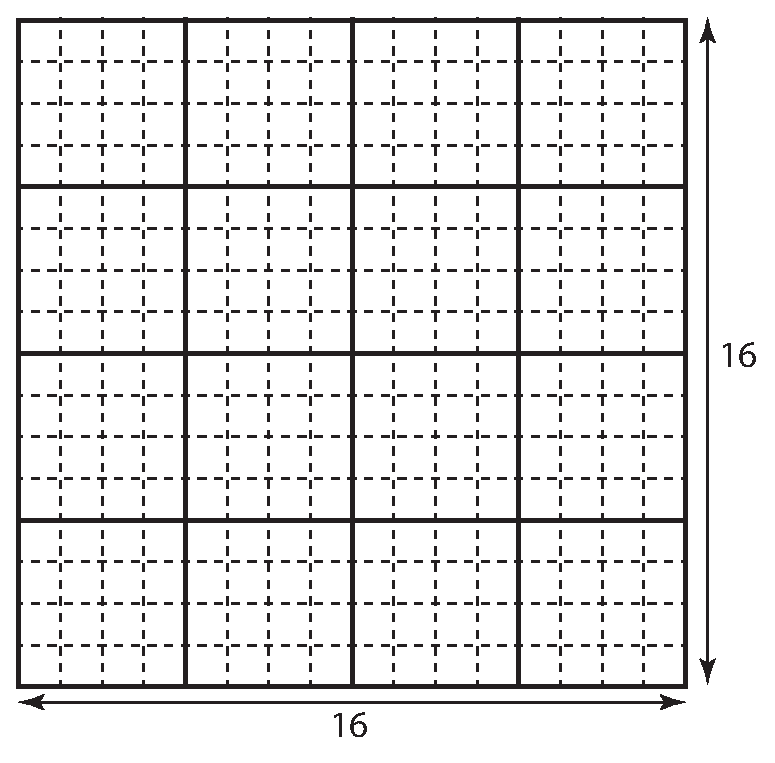
\includegraphics{quadtree/images/qdt_initial_mesh.eps}
    }
    \caption{An example of the background initial mesh: $16 \times 16$ square are divided into $2^4 \times 2^4$ pixels (dashed lines, $res=4$) and $2^2 \times 2^2$ pixels form the initial mesh (solid lines, $s_{max}=2$)}
    \label{qdt_fig:qdt_initial_mesh}
\end{figure}

\paragraph{}
% generating the initial mesh without balance
Criteria to decided whether each individual square in the initial mesh need to be refined or not is the seed points.
The curve will be uniformly discretized into a given number of seed points uniformly and the mesh will be refined until the number of the seed points within the square is less than the threshold.
However, finer mesh is expected at the region where geometry with high curvature appeared but the uniform discretization does not generate different number of points based on curvature.
It can be solved by treating each segment of the polylines as an individual curve when generating seed points.
Due to the fact that algorithm described in .~\ref{qdt_section:iges_output} guarantee the chord length to arc length ratio, polylines ought to have finer segments at the position where curvature is significant.

\paragraph{}
% only two intersections allowed
Although seed points provides a good guide on the mesh density, situations where high density mesh is required while few seed points appeared may happen as plotted in fig.~\ref{qdt_fig:qdt_seed_point_problem}.
The geometry limits the seed points due to the lack of curvature.
While, it is expected that the square element will be refined at least once as one layer of mesh may not be appropriate to formulate a thin shell structure. 
    \begin{figure}[!ht]
        \centering
        \scalebox{1}{
            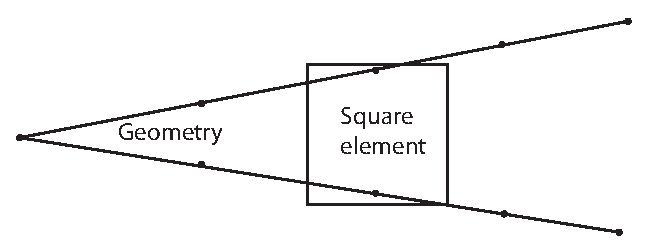
\includegraphics{quadtree/images/qdt_seed_points_problem}
        }
        \caption[Limitation of the seed points]{
            Limitation of the seed points: few seed points will be generated over a straight line and few seed points will be included in the square element which leads to unexpected behavior.
            \tikz\draw[black,fill=black] (0,0) circle (.7ex);
            stands for the seed points.
        }
        \label{qdt_fig:qdt_seed_point_problem}
    \end{figure}
As a result, another restriction will be adopted together with the seed points to prevent this kind of situation from happening.
Element with more than two unique intersections will be tagged to be refined no matter how many seed points it contains.
In numerical calculation, two points may be regarded as one if they are close enough to each others.
Normalization of the geometry described at the beginning of this section helps to define a meaningful tolerance to handle numerical error.



% balance the initial mesh
\paragraph{}
% balance in tree data structure
Self-balancing is adopted by most of the tree data structure such as AVL, B/B+, Red-black tree and so on.
Fig.~\ref{qdt_fig:tree_balance_avl} illustrates a self-balancing of an AVL tree.
Balancing by rotation is performed because difference in height of the leaf B and L is greater than the threshold.
    \begin{figure}
        \centering
        \scalebox{0.25}{
            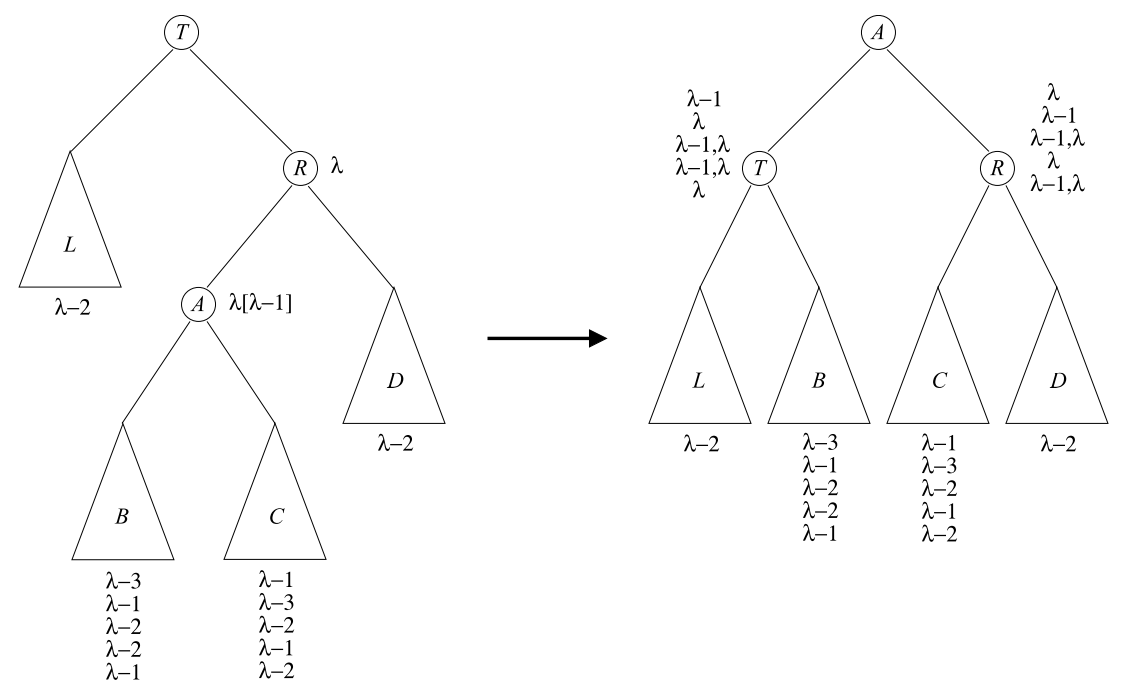
\includegraphics{quadtree/images/qdt_avl_balance.png}
        }
        \caption{Balance of the AVL tree \cite{Roura2013}}
        \label{qdt_fig:tree_balance_avl}
    \end{figure}

\paragraph{}
% balance in quadtree
Same idea is adopted in quadtree as well.
a refinement will be performed to achieve a balanced tree if the difference in the height of the leaf (Cell A and B in fig.~\ref{qdt_fig:tree_balance_quadtree} for example) is larger than one.
    \begin{figure}[!ht]
        \begin{subfigure}[b]{0.5\linewidth}
            \centering
            \scalebox{0.8}{
                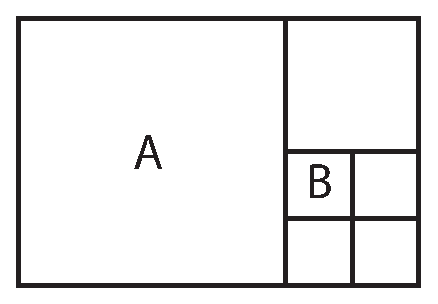
\includegraphics{quadtree/images/qdt_balance_before.eps}
            }
            \caption{Before balance operation}
        \end{subfigure}
        \begin{subfigure}[b]{0.5\linewidth}
            \centering
            \scalebox{0.8}{
                
\includegraphics{quadtree/images/qdt_balance_after.eps}
            }
            \caption{After balance operation}
        \end{subfigure}
        \caption{Balance of quadtree: cell A is refined in order to balance the quadtree.}
        \label{qdt_fig:tree_balance_quadtree}
    \end{figure}

\paragraph{}
% reason behind balancing
The reason why balancing is predominately adopted in tree data structure lies in the guarantee of an $O\left(log(n)\right)$ time complexity for searching in any case.
Even thought computational cost on searching seems not to be significant during mesh generation using quadtree, a balanced tree provided some other attractive features that can be utilized in numerical analysis.
One of the advantages is to improve the mesh quality.
Any extremely small or large angle between the element and the scaling center may result in a bad quality mesh.
Chances are that these poor quality mesh may appear without self-balancing, fig.~\ref{qdt_fig:sbfem_adv_1} for an example.
    \begin{figure}[!ht]
        \centering
        \scalebox{1}{
            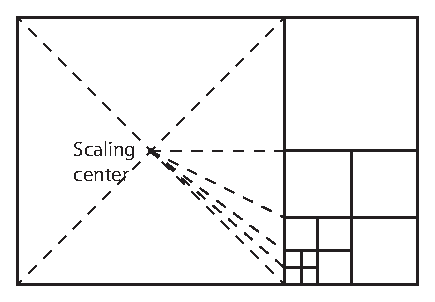
\includegraphics{quadtree/images/qdt_balance_sbfem_adv_1.eps}
        }
        \caption{Small angle between element and scaling center may reduce the mesh quality}
        \label{qdt_fig:sbfem_adv_1}
    \end{figure}

Another reason is to kept the pattern of the cells.
If the threshold of the self-balancing is set to one ($2:1$ ratio), only six kinds of cells will appear before the cutting as illustrated in fig.~\ref{qdt_fig:sbfem_adv_2}.
Thanks to the geometric similarity, local stiffness matrix can be calculated and scaled directly when same kind of the cell appears which significantly reduce the computational cost.
Hanging nodes in fig.~\ref{qdt_fig:sbfem_adv_2} can be a problem for traditional finite element to handle the displacement compatibility \cite{Tabarraei:2009:XFE} \cite{NME:NME3070} \cite{NME:NME2900} .
Solution including triangulation \cite{4037344} \cite{BERN1994384} \cite{ijeas251083} , using special shape function \cite{NME:NME1620120104} and other methods are available but special treatment is required.
As a comparison, SBFEM provides greater flexibility on the element, n-sides polygons with hanging nodes or curved edge can be treated natively.
    \begin{figure}[!ht]
        \centering
        \scalebox{1}{
            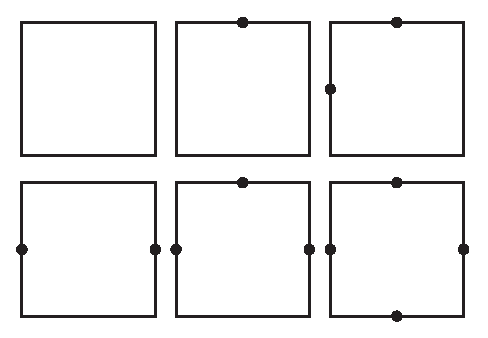
\includegraphics{quadtree/images/qdt_balance_sbfem_adv_2.eps}
        }
        \caption[Types of the cell in self-balancing quadtree]{
            Types of the cell when $2:1$ ratio is applied,
            \tikz\draw[black,fill=black] (0,0) circle (.7ex);
            stands for the hanging node
            }
        \label{qdt_fig:sbfem_adv_2}
    \end{figure}


\pagebreak


%=====================================================================================================================%
\subsection{Hard point treatment}
\paragraph{}
%introduction
Hard point is a kind of point in the geometry that must be meshed as a node or scaling center.
When more than two materials are involved, it is common to have some hard points to make sure the point shared by three material can be properly formulated as shown in fig.~\ref{qdt_fig:qdt_hard_point_demo}
    \begin{figure}[!ht]
        \begin{subfigure}[b]{0.5\linewidth}
            \centering
            \scalebox{0.8}{
                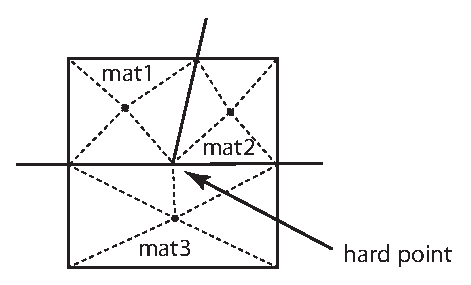
\includegraphics{quadtree/images/qdt_hard_point_demo.eps}
            }
        \caption{Hard point is meshed as node}
        \end{subfigure}
        \begin{subfigure}[b]{0.5\linewidth}
            \centering
            \scalebox{0.8}{
                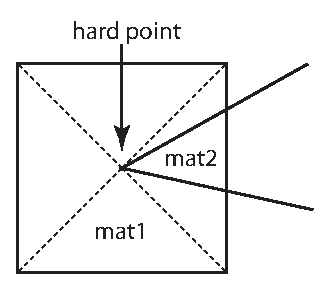
\includegraphics{quadtree/images/qdt_hard_point_demo_2.eps}
            }
        \caption{hard point is meshed as scaling center}
        \label{qdt_fig:qdt_hard_point_demo_sc}
        \end{subfigure}
        \caption[Example of a hard point]{Example of a hard point, elements around the point shared by three material must be properly divided into three.}
        \label{qdt_fig:qdt_hard_point_demo}
    \end{figure}
The difficulty in treating a hard point will be the position of itself in the background mesh.
The further it is away from the geometric center of the background mesh, the poorer the quality of mesh will be generated.
If the hard point in fig.~\ref{qdt_fig:qdt_hard_point_demo_sc} is located somewhere that is very close to the left boundary of the background mesh, the mesh for material one after cutting may be a quite elongated and twisted concave unit.
Besides, the requirement of the scaling center in the SBFEM can always be satisfied no matter where it is located in a convex polygon.
The opposite is true for a concave polygon, special treatment must be adopted to fullfil this requirement.
As a consequence, generally speaking, a convex mesh may always be preferred over a concave one and hard point can be the only source that will introduce concave polygons in most of the situation.
Although algorithm finding qualified scaling center in a concave polygon exists, the quality of the mesh may not be satisfactory even the scaling center is located on the vertex.


\paragraph{}
% make sure the hard point is close to the center of the background mesh
The first step to treat the hard point will be trying to locate the background mesh so that the hard point is close enough to its geometric center.
The ideal size of the background mesh shall ensure that only one hard point is in it and that no points from any other curves should be located in it.
As a consequence, the size of the containing square $box\_size$ is set to be one third of the distance to the nearest curves or half of the distance to the nearest hard point, whichever is smaller.
These parameter usually result in a valid and large enough background mesh that can treat the hard point easily. 
When building the background cell containing hard point in the algorithm, it will be implemented by have a considerably fine mesh within the range of the hard point and merge all cells in that range into one larger cell to be the background one.
Size of the ``considerably fine'' mesh $size\_field$ will be defined with the adjacent vertexes of the hard point as in eq.~\ref{qdt_eq:qdt_hard_point_size_field}
    \begin{equation}
        size\_field = \frac{box\_size}{
            2^{
                round(
                    \log(\frac{2 \pi}{ min(\alpha)})-1
                )
            }
        }
    \label{qdt_eq:qdt_hard_point_size_field}
    \end{equation}
where $\alpha$ is the minimal angle $min(\alpha_1, \alpha_2, \dots, \alpha_n)$ in fig.~\ref{qdt_fig:qdt_hard_point_setp_1}.
As is exponentially related to the minimal angle $\alpha$, the $size\_field$ may always be small enough to capture thin shell.
    \begin{figure}
        \centering
        \scalebox{0.5}{
            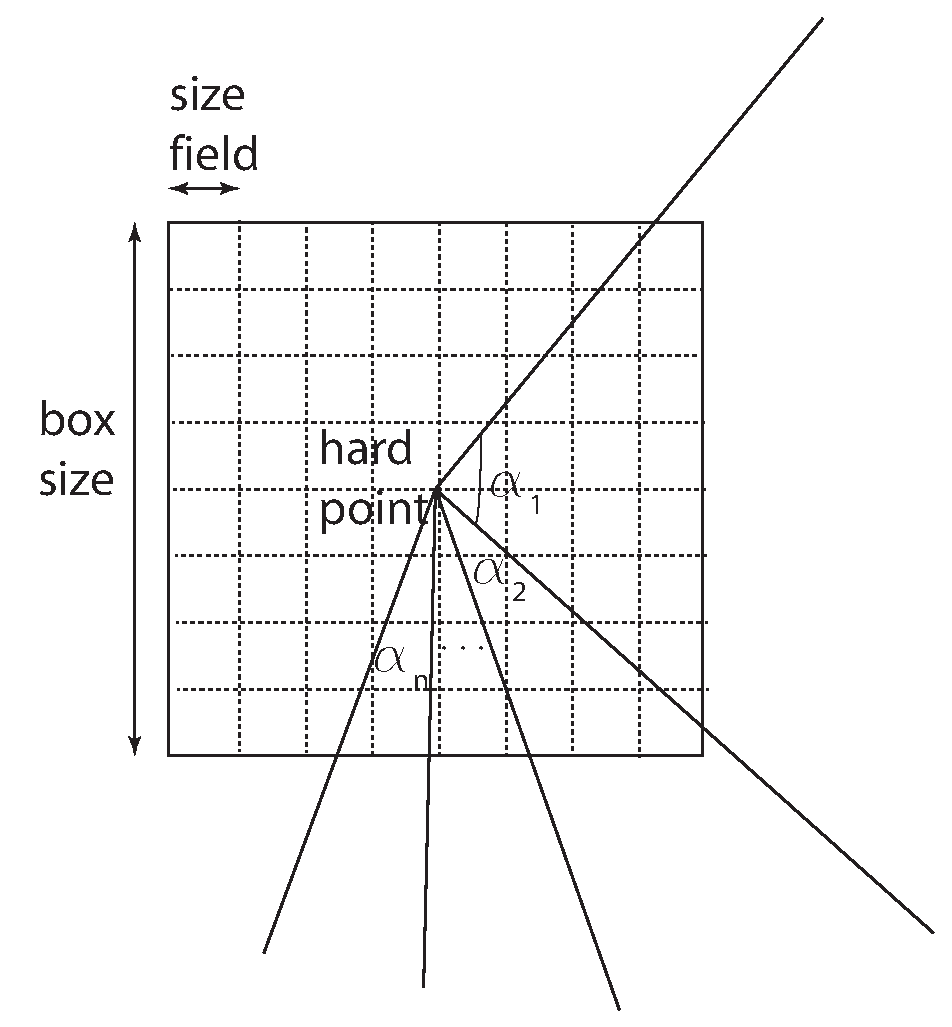
\includegraphics{quadtree/images/qdt_hard_point_step_1.eps}
        }
        \caption[Hard point treatment step 1]{Hard point treatment step1: find $box\_size$ and $size\_field$}
        \label{qdt_fig:qdt_hard_point_setp_1}
    \end{figure}

After the first step of the hard point treatment is done, the background cell shall have the following properties
    \begin{enumerate}
        \item Distance between hard point to geometric center of the background cell must be smaller than $\sqrt{2}size\_field$
        \item Element after cutting share the hard point as the node or it will be one element with scaling center located at the hard point
    \end{enumerate}
With these two properties, the cell can be cut by simply connecting the intersections with the hard point later.
\pagebreak


%=====================================================================================================================%
\subsection{Bucket sort algorithm}



\pagebreak
%=====================================================================================================================%
\subsection{Cutting with boundary}



\pagebreak
%=====================================================================================================================%
\subsection{Scaling center for concave elements}



\pagebreak
%=====================================================================================================================%
\subsection{Color the region}



\pagebreak

% \section{NURBS utilization}
% \label{qt_sc:nurbs}
% \input{quadtree/nurbs.tex}


\section{Numerical Examples}
\subsection{Cantilever beam}
\paragraph{}
A two-dimensional cantilever beam subjected to a parabolic shear load at the free end is examined as shown
in fig.~\ref{qdt_fig:ex_cantilever_beam_geo_bc}.
    \begin{figure}[h!]
    \centering
        \scalebox{0.8}{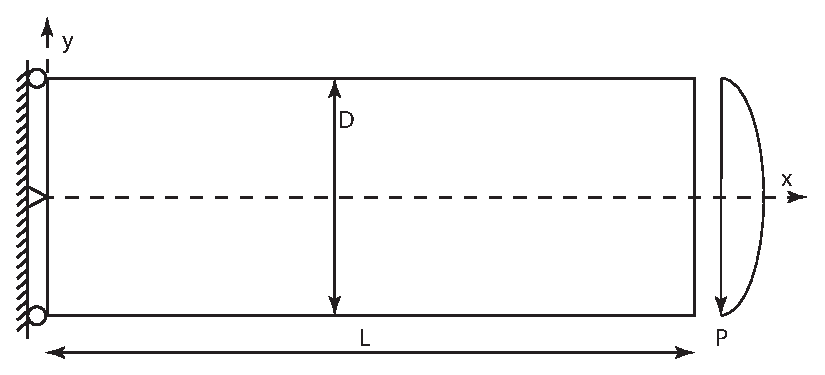
\includegraphics{isogeometric_sbfem/images/cantilever_beam_geo_bc.eps}}
        \caption{ Cantilever beam: Geometry and boundary conditions.}
        \label{qdt_fig:ex_cantilever_beam_geo_bc}
    \end{figure}

The geometry is: length $L=8m$, height $D=4m$.
The material properties are: Young’s modulus $E$ = $3 \times 10^7 N/m^2$ , Poisson’s ratio $ \nu =0.25$.
The parabolic shear force is $P = 250 N$.
The exact solutions for the displacements are given by \cite{Aug2008} as eq.~\ref{iso_eq:cantilever_beam_displacement_solution}.
where $I=D^3/12$ is the moment of inertia, $\mean{E}=E$, $\mean{\nu}=\nu$ and $\mean{E}=E/(1-\nu^2)$, $\mean{\nu}=nu/(1-nu)$ for plane stress and plane strain condition respectively.
The stress $\sigma$ can be expressed as \cite{Aug2008} as eq.~\ref{iso_eq:cantilever_beam_stress_solution}.
The strain energy can be derived from eq.~\ref{iso_eq:cantilever_beam_stress_solution} and eq.~\ref{iso_eq:cantilever_beam_displacement_solution} as eq.~\ref{iso_eq:cantilever_beam_energy_solution}.

\paragraph{}
In this example, rigid body motion is constrained by fixing 3 DOF on the left edge of the beam.
$u_x=0$ for points at $(0,-D/2)$ and $(0,D/2)$ and $u_y =0$ for point at $(0,0)$.
Stress from analytical solution in eq.~\ref{iso_eq:cantilever_beam_stress_solution} are applied on the boundary.

\paragraph{}
Due to the fact that the geometry of the cantilever beam can be described by four points and four straight lines, drawing in AutoCAD may not be necessary.
As a result, the input geometry is defined manually.
Generated background mesh, coloring and the final result with $res=32$, $s_{max}=16$ and $s_{min}=1$ are shown in fig.~\ref{qdt_fig:ex_cantilever_beam_background_mesh}, fig.~\ref{qdt_fig:ex_cantilever_beam_mesh_coloring} and fig.~\ref{qdt_fig:ex_cantilever_beam_mesh_final}.

    \begin{figure}
        \centering
        \scalebox{0.6}{
            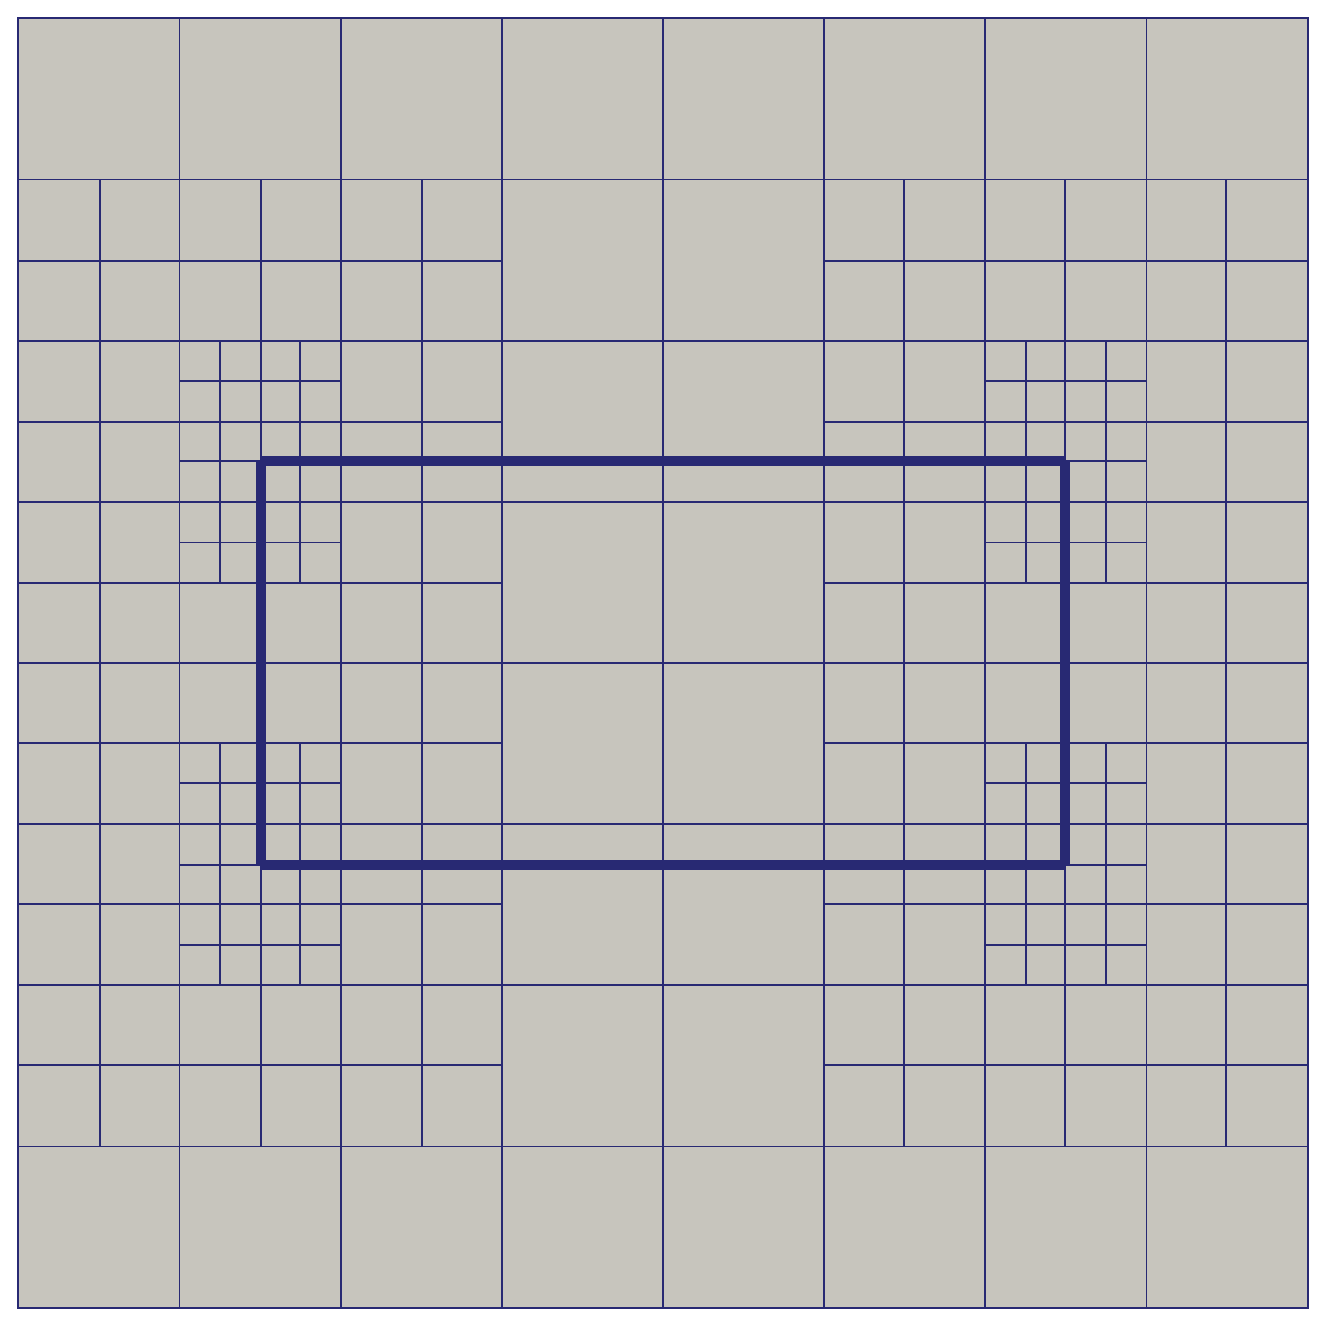
\includegraphics{quadtree/ex_images/cantilever_background_mesh.eps}
        }
        \caption[Background mesh of cantilever beam]{Background mesh of cantilever beam : Bold lines represents the input geometry}
        \label{qdt_fig:ex_cantilever_beam_background_mesh}
    \end{figure}

    \begin{figure}
        \centering
        \scalebox{0.6}{
            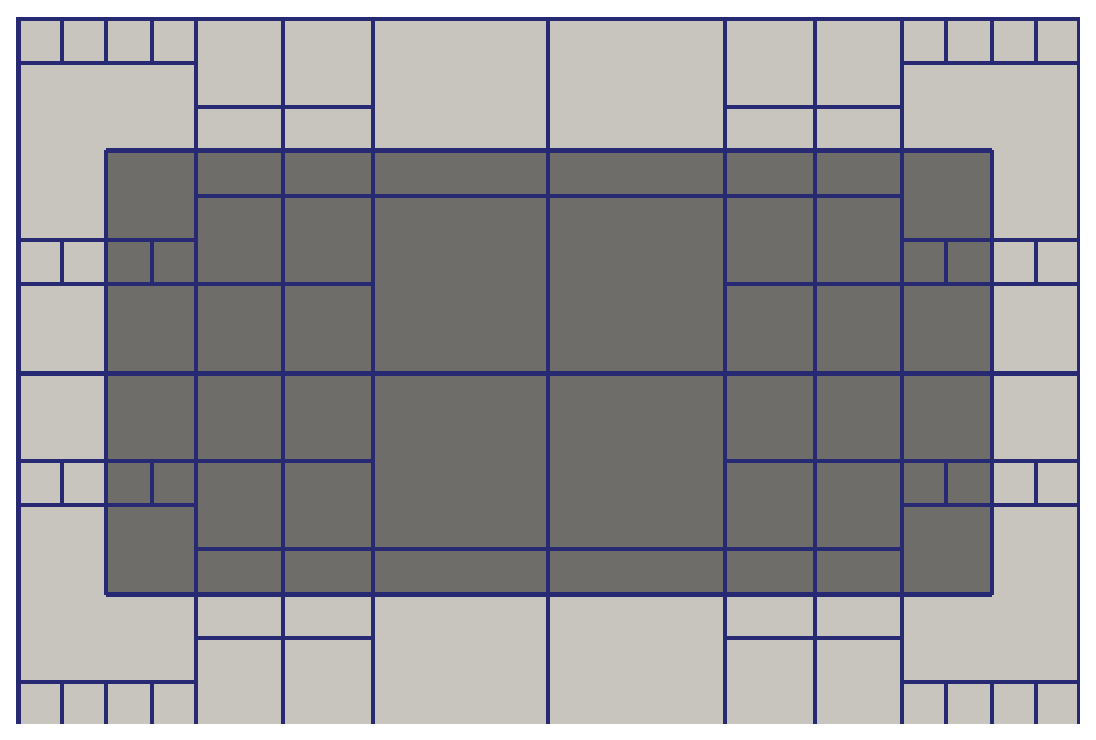
\includegraphics{quadtree/ex_images/cantilever_coloring.eps}
        }
        \caption[Mesh coloring of cantilever beam]{Mesh coloring of cantilever beam : Grey area represents the cantilever beam}
        \label{qdt_fig:ex_cantilever_beam_mesh_coloring}
    \end{figure}

    \begin{figure}
        \centering
        \scalebox{0.5}{
            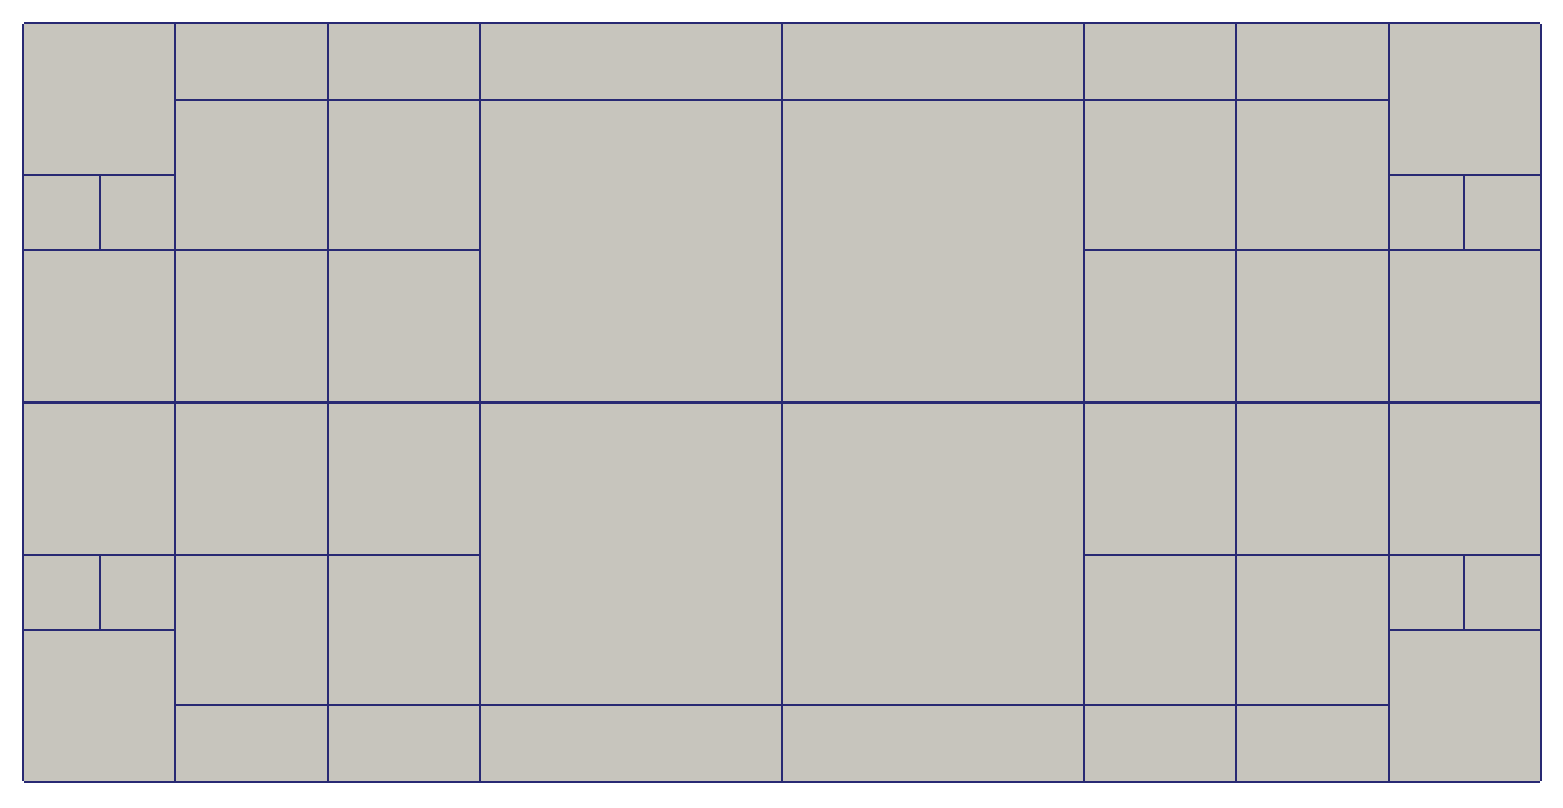
\includegraphics{quadtree/ex_images/cantilever_final_mesh.eps}
        }
        \caption[Final mesh of cantilever beam]{Final mesh of cantilever beam}
        \label{qdt_fig:ex_cantilever_beam_mesh_final}
    \end{figure}
% DOF err
% 146 - 0.019587 (32,16)
% 178 - 0.0082845 (32,2)
% 438 - 0.0027044 (64,2)
% 1658- 0.00066929 (128,2)
\paragraph{}
Mesh with different parameters are plotted in fig.~\ref{qdt_fig:ex_cantilever_mesh_all} and the convergence study is plotted in fig.~\ref{qdt_fig:ex_cantilever_mesh_conv}

    \begin{figure}[!ht]
        \begin{subfigure}[b]{1\linewidth}
            \centering
            \scalebox{0.4}{
                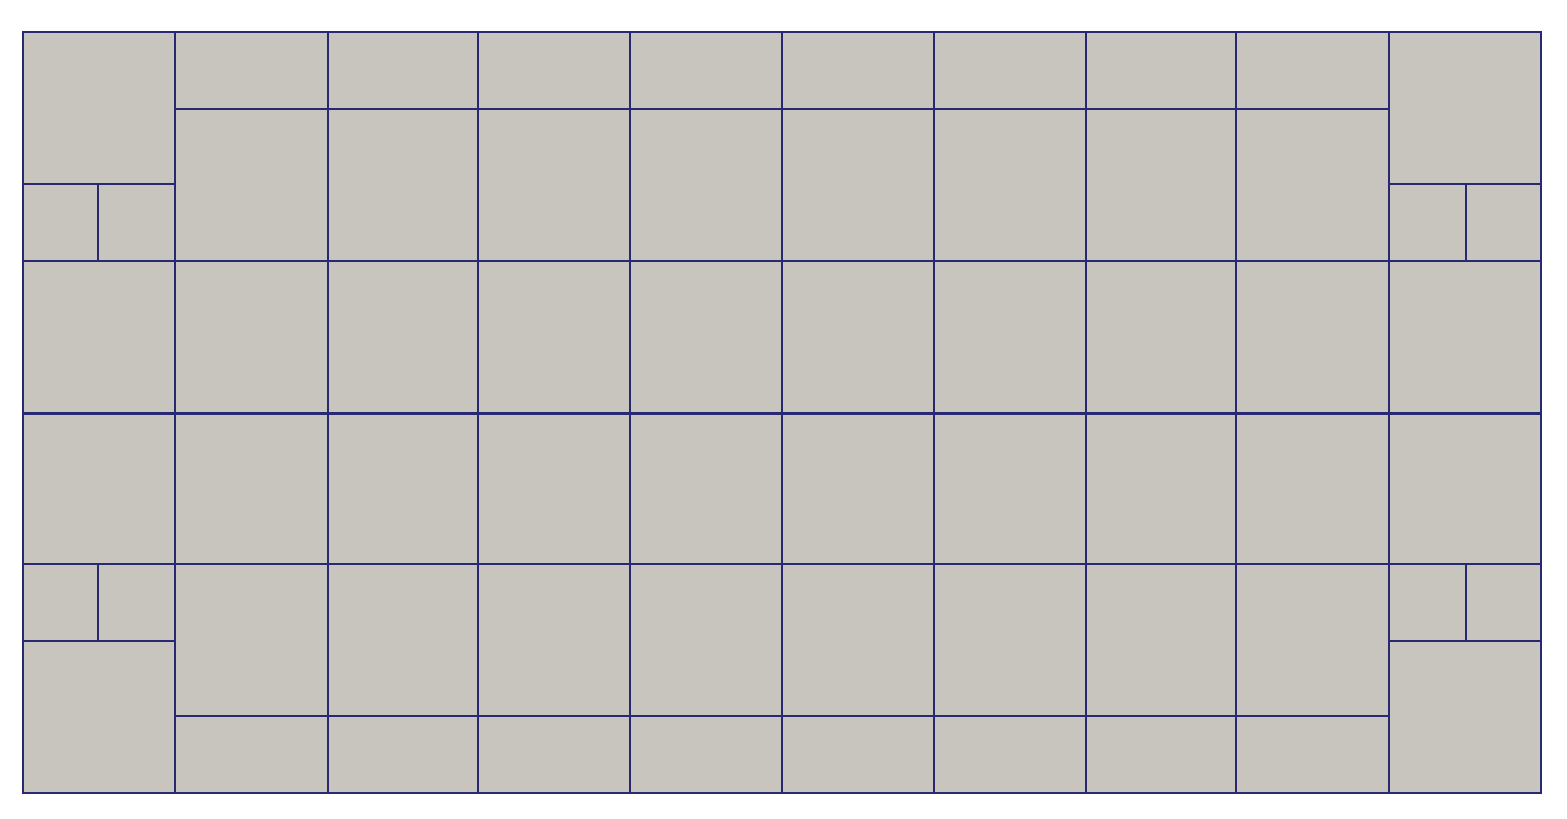
\includegraphics{quadtree/ex_images/qdt_cantilever_mesh_178.eps}
            }
            \caption{Mesh with $res=32$, $s_{max}=2$, 178 DOFs}
        \end{subfigure}
        \\
        \begin{subfigure}[b]{1\linewidth}
            \centering
            \scalebox{0.4}{
                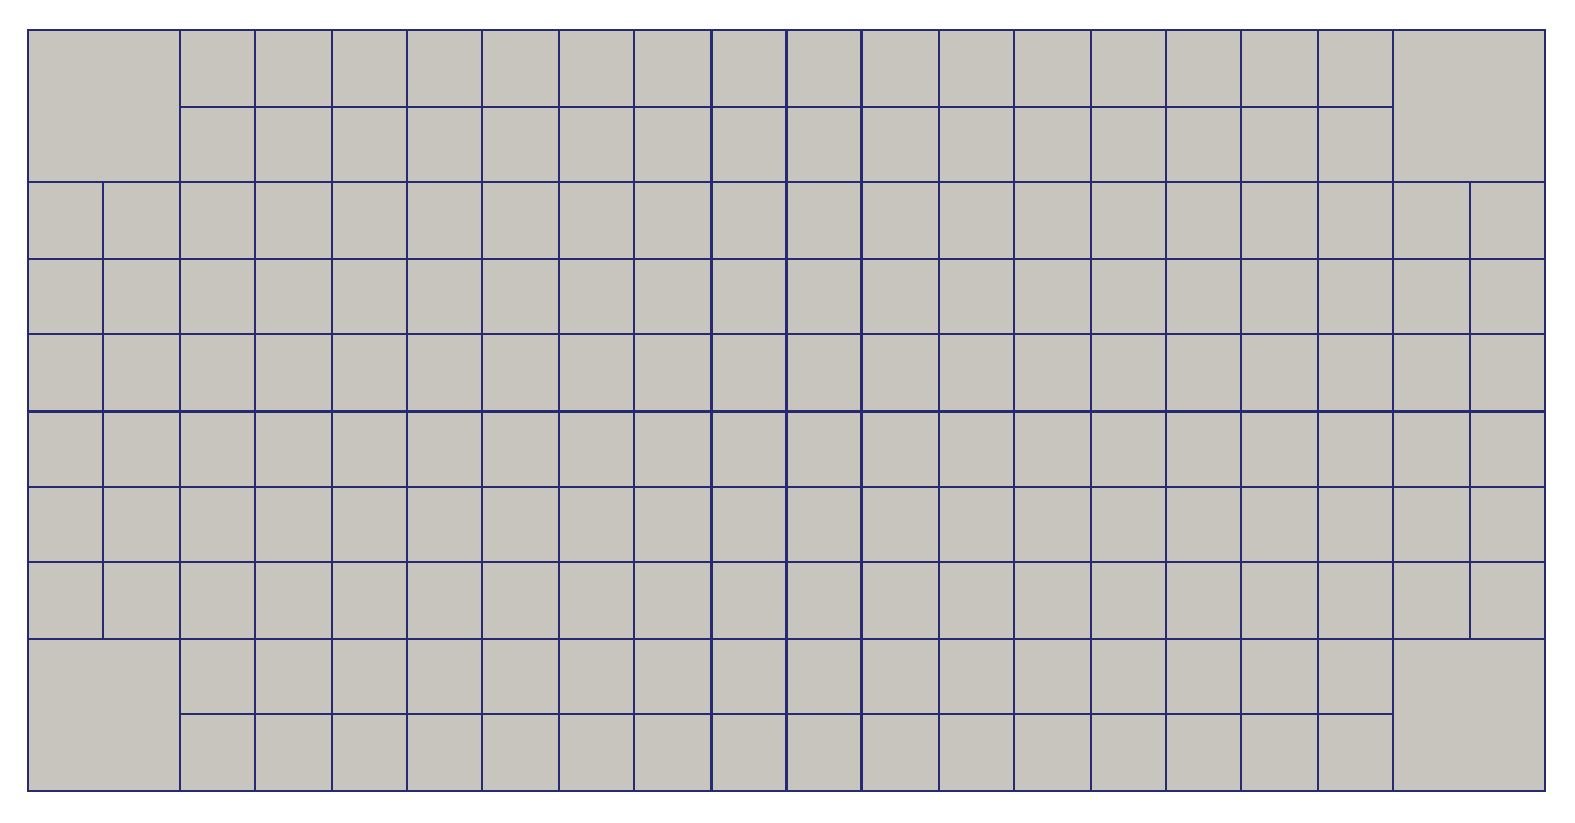
\includegraphics{quadtree/ex_images/qdt_cantilever_mesh_438.eps}
            }
            \caption{Mesh with $res=64$, $s_{max}=2$, 438 DOFs}
        \end{subfigure}
        \\
        \begin{subfigure}[b]{1\linewidth}
            \centering
            \scalebox{0.4}{
                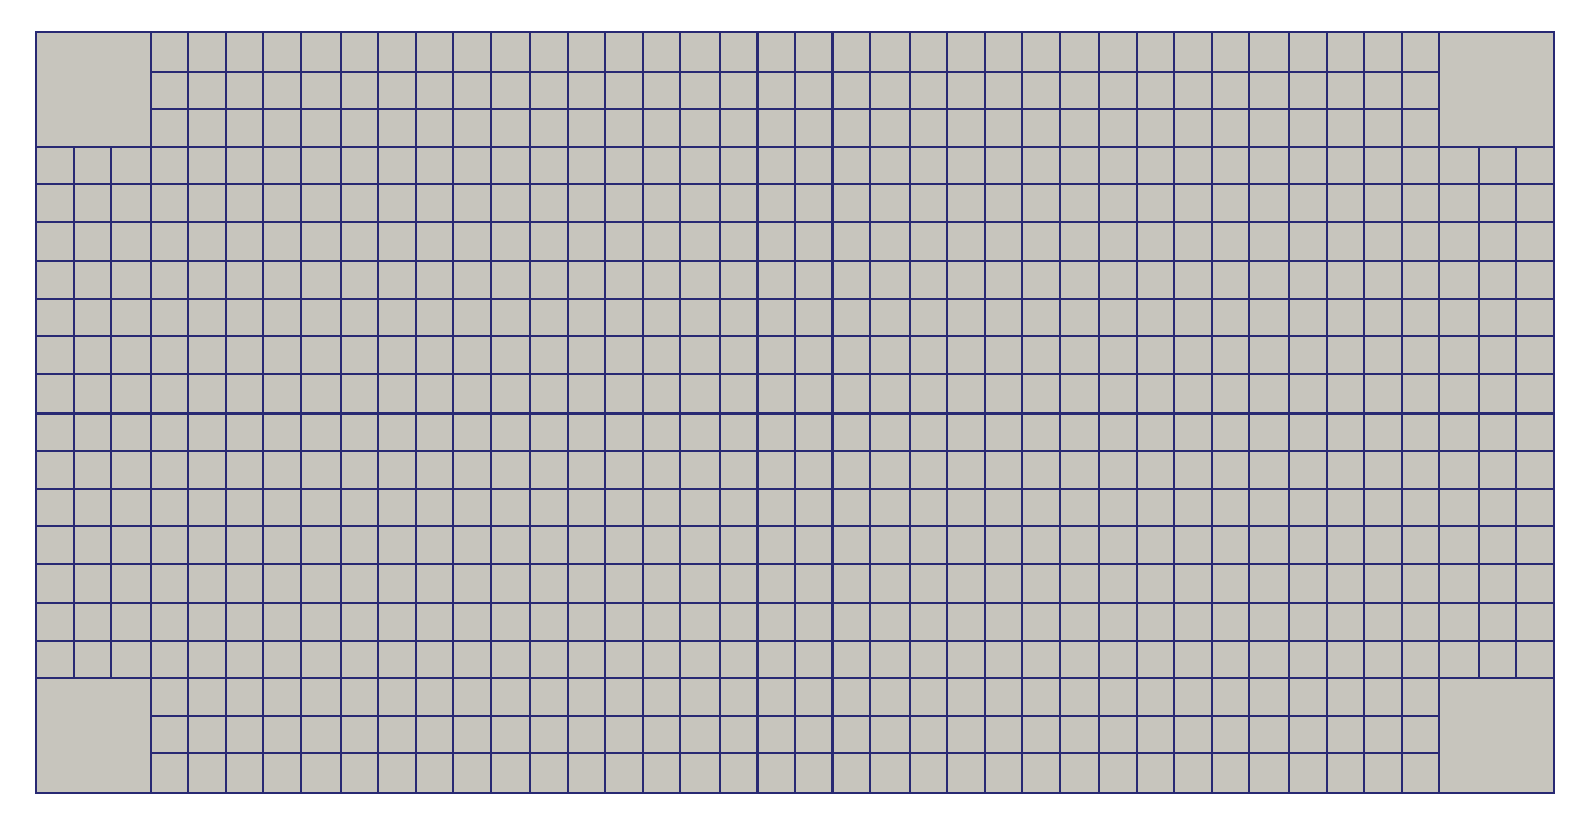
\includegraphics{quadtree/ex_images/qdt_cantilever_mesh_1658.eps}
            }
            \caption{Mesh with $res=128$, $s_{max}=2$, 1658 DOFs}
        \end{subfigure}
        \caption[Mesh of the cantilever beam]{Mesh of the cantilever beam}
        \label{qdt_fig:ex_cantilever_mesh_all}
    \end{figure}


    \begin{figure}[H]
        \centering
        \scalebox{0.75}{
            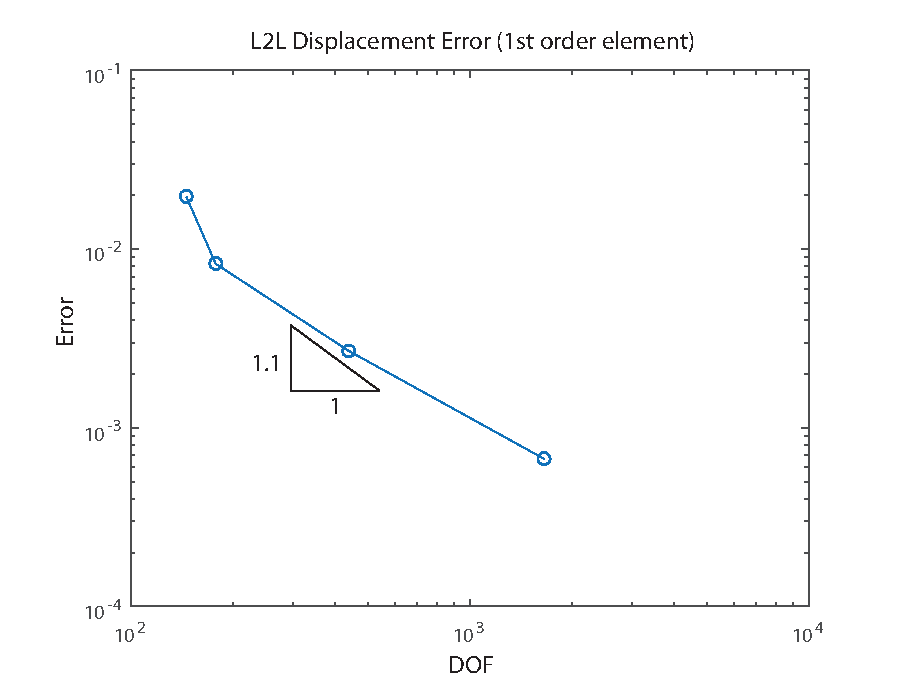
\includegraphics{quadtree/ex_images/qdt_cantilever_conv.eps}
        }
        \caption[Convergence of the cantilever beam]{Convergence of the cantilever beam}
        \label{qdt_fig:ex_cantilever_mesh_conv}
    \end{figure}

    
\pagebreak
\subsection{Infinite plate with a circular hole}
\paragraph{}
In this example, an infinite plate with a traction free hole under uniaxial tension $(\sigma = 1 N/m^2 )$ along x-axis (see Fig.~\ref{qdt_fig:ex_chole_geo_bc}) is considered.
$L$ is taken as $20$ and $r$ is $5$.
The material properties are: Young’s modulus $E = 100 N/m^2$ and Poisson’s ratio $\nu = 0.3$.
    \begin{figure}[H]
        \centering
        \scalebox{0.5}{
            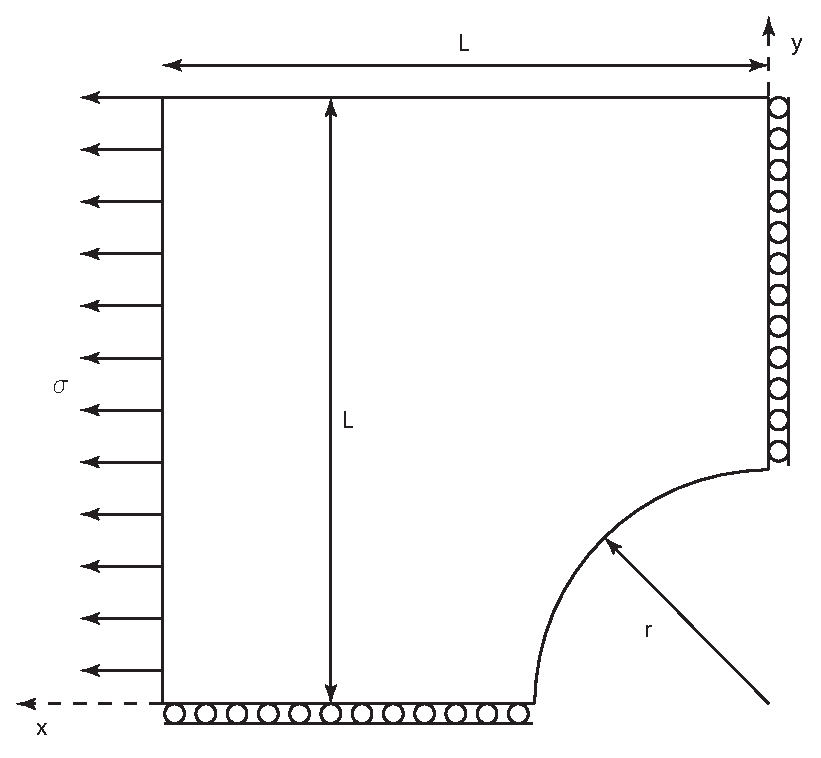
\includegraphics{quadtree/ex_images/qdt_chole_quat_geo_bc.eps}
        }
        \caption{ Infinite plate with a circular hole: geometry and boundary conditions}
        \label{qdt_fig:ex_chole_geo_bc}
    \end{figure}
%
The exact solution of the principal stresses in Cartesian coordinate $(r,\theta)$ is given by \cite{Sukumar2001} in Eq.~\ref{iso_eq:ex_chole_stress_sol}.
The closed form displacement in Cartesian coordinate is given in Eq.~\ref{iso_eq:ex_chole_disp_sol}.
\paragraph{}
Geometry of the example will be extracted from the iges file drawn in AutoCAD (Fig.~\ref{qdt_fig:ex_chole_cad}).
    \begin{figure}[H]
        \centering
        \scalebox{0.35}{
            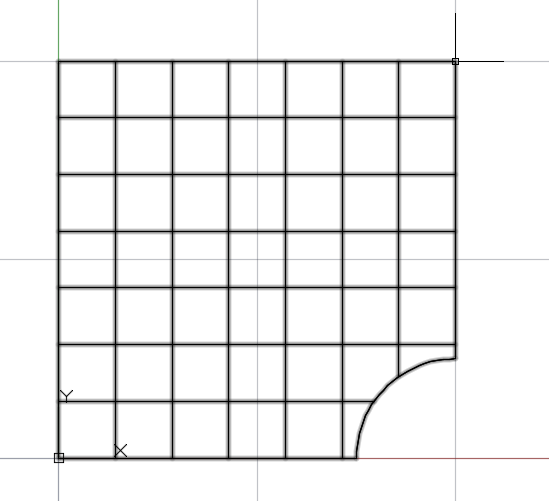
\includegraphics{quadtree/ex_images/ex_chole_cad.png}
        }
        \caption{Infinite plate with a circular hole: CAD drawing}
        \label{qdt_fig:ex_chole_cad}        
    \end{figure}
%
Generated background mesh, coloring and the final result with $res=32$, $s_{max}=4$ and $s_{min}=1$ are shown in Fig.~\ref{qdt_fig:ex_chole_background_mesh}, Fig.~\ref{qdt_fig:ex_chole_mesh_coloring} and Fig.~\ref{qdt_fig:ex_chole_mesh_final}.

\begin{figure}
    \centering
    \scalebox{0.35}{
        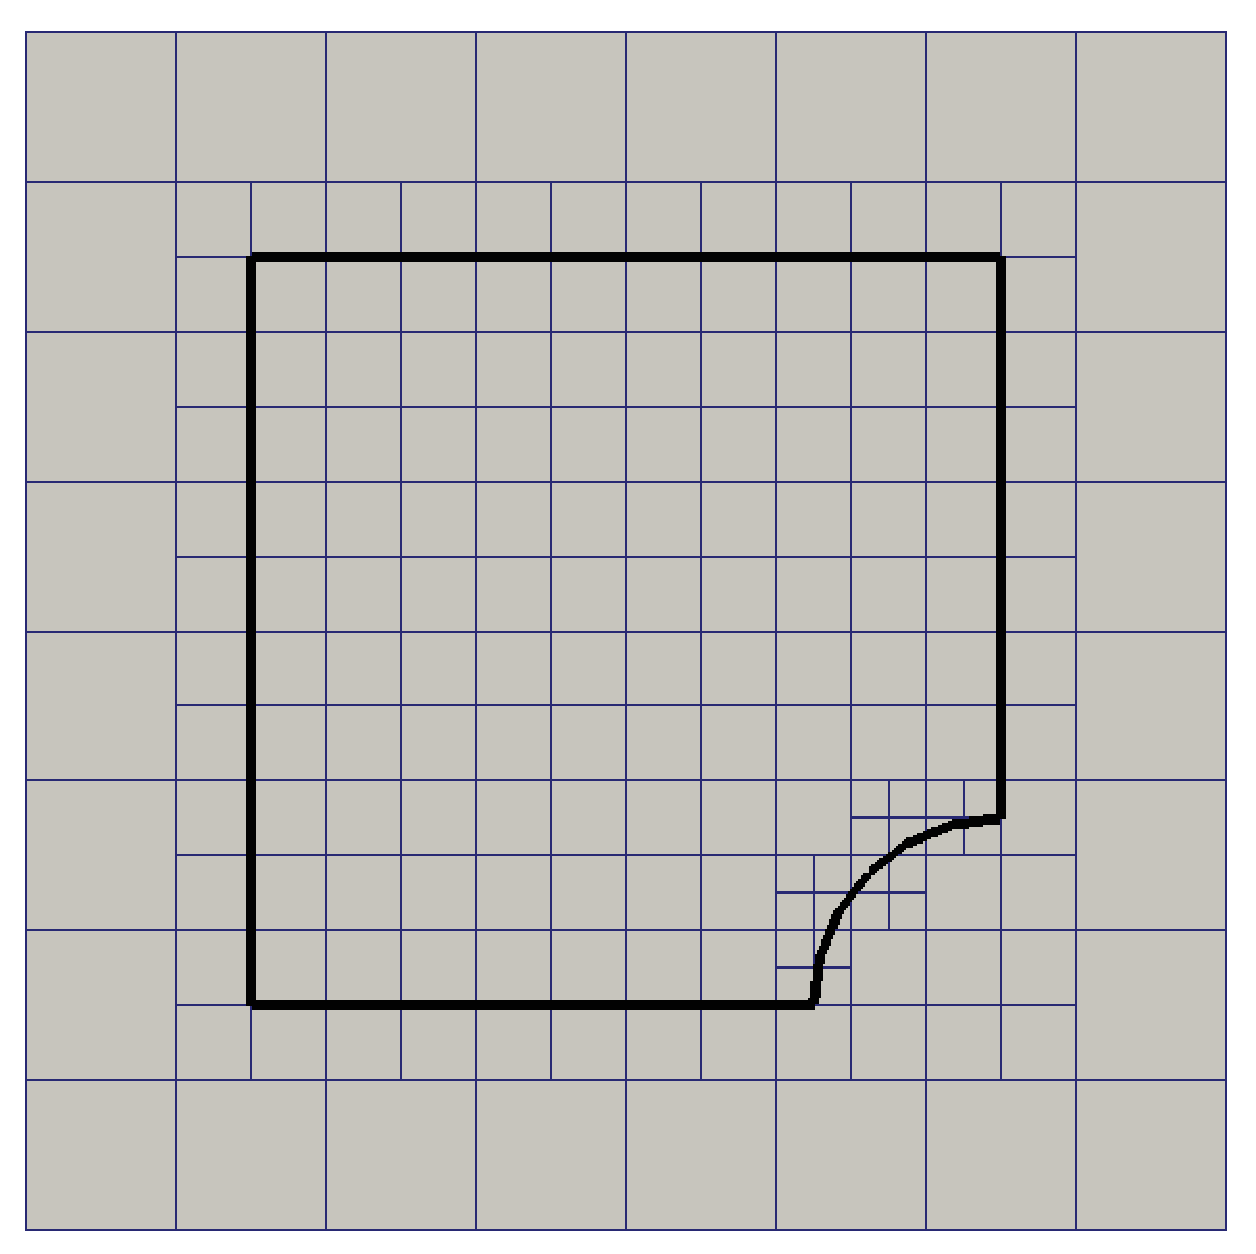
\includegraphics{quadtree/ex_images/ex_chole_background.eps}
    }
    \caption[Background mesh of infinite plate with a circular hole]{Background mesh of infinite plate with a circular hole : Bold lines represents the input geometry}
    \label{qdt_fig:ex_chole_background_mesh}
\end{figure}

\begin{figure}
    \centering
    \scalebox{0.35}{
        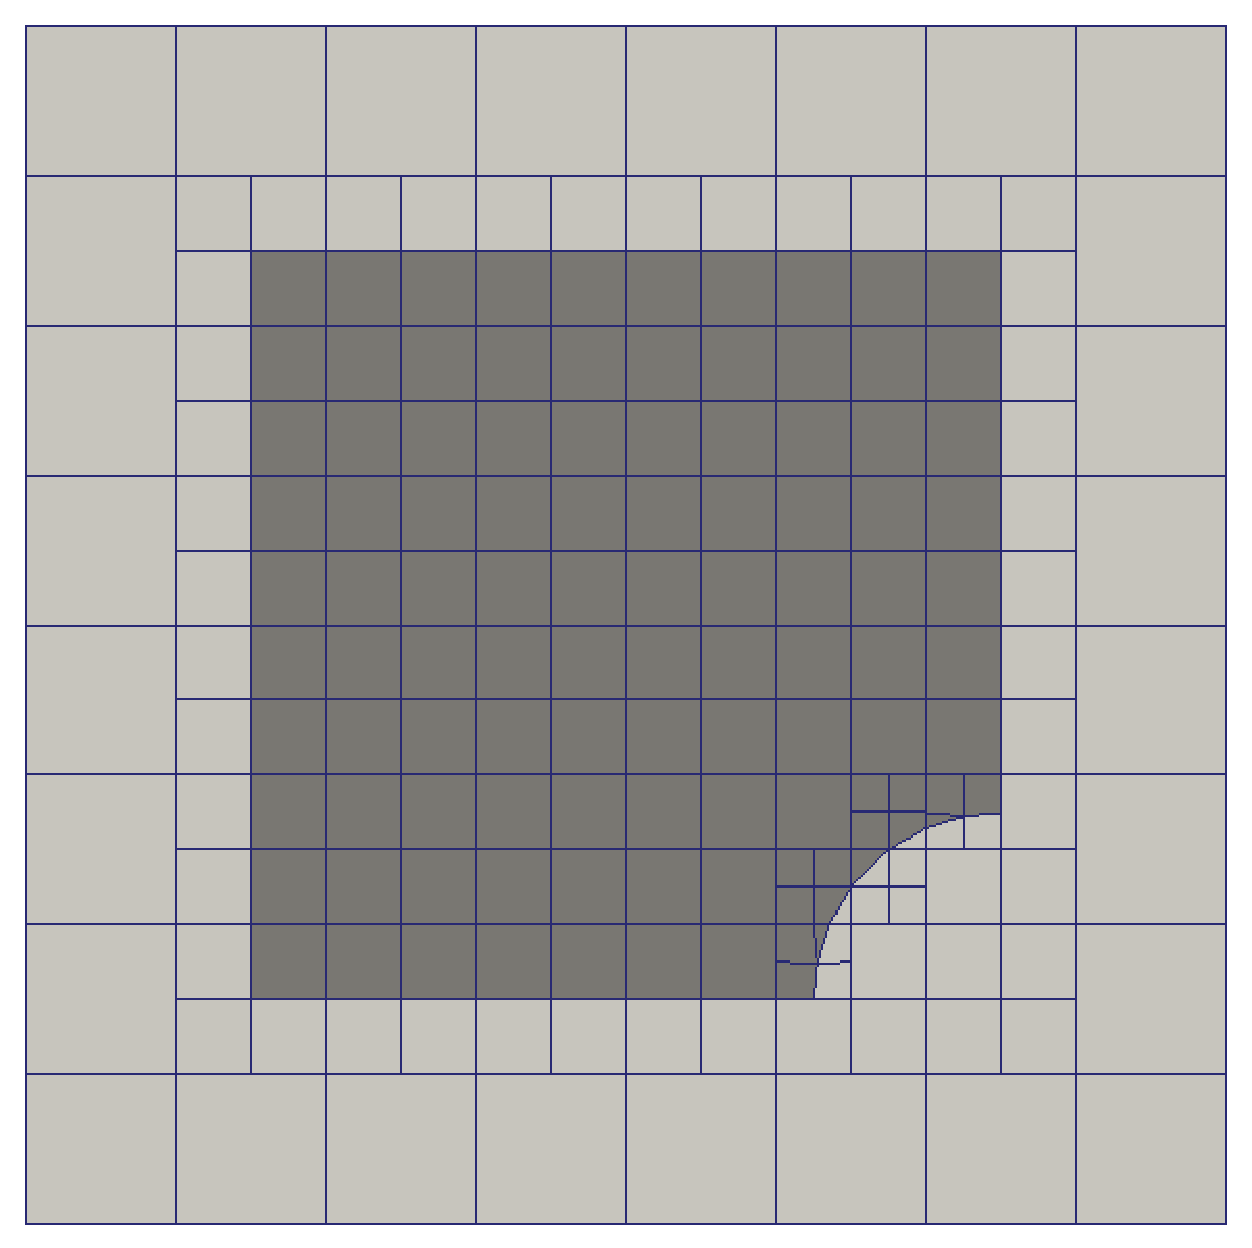
\includegraphics{quadtree/ex_images/ex_chole_coloring.eps}
    }
    \caption[Mesh coloring of infinite plate with a circular hole]{Mesh coloring of infinite plate with a circular hole : Grey area represents the plate}
    \label{qdt_fig:ex_chole_mesh_coloring}
\end{figure}

\begin{figure}
    \centering
    \scalebox{0.35}{
        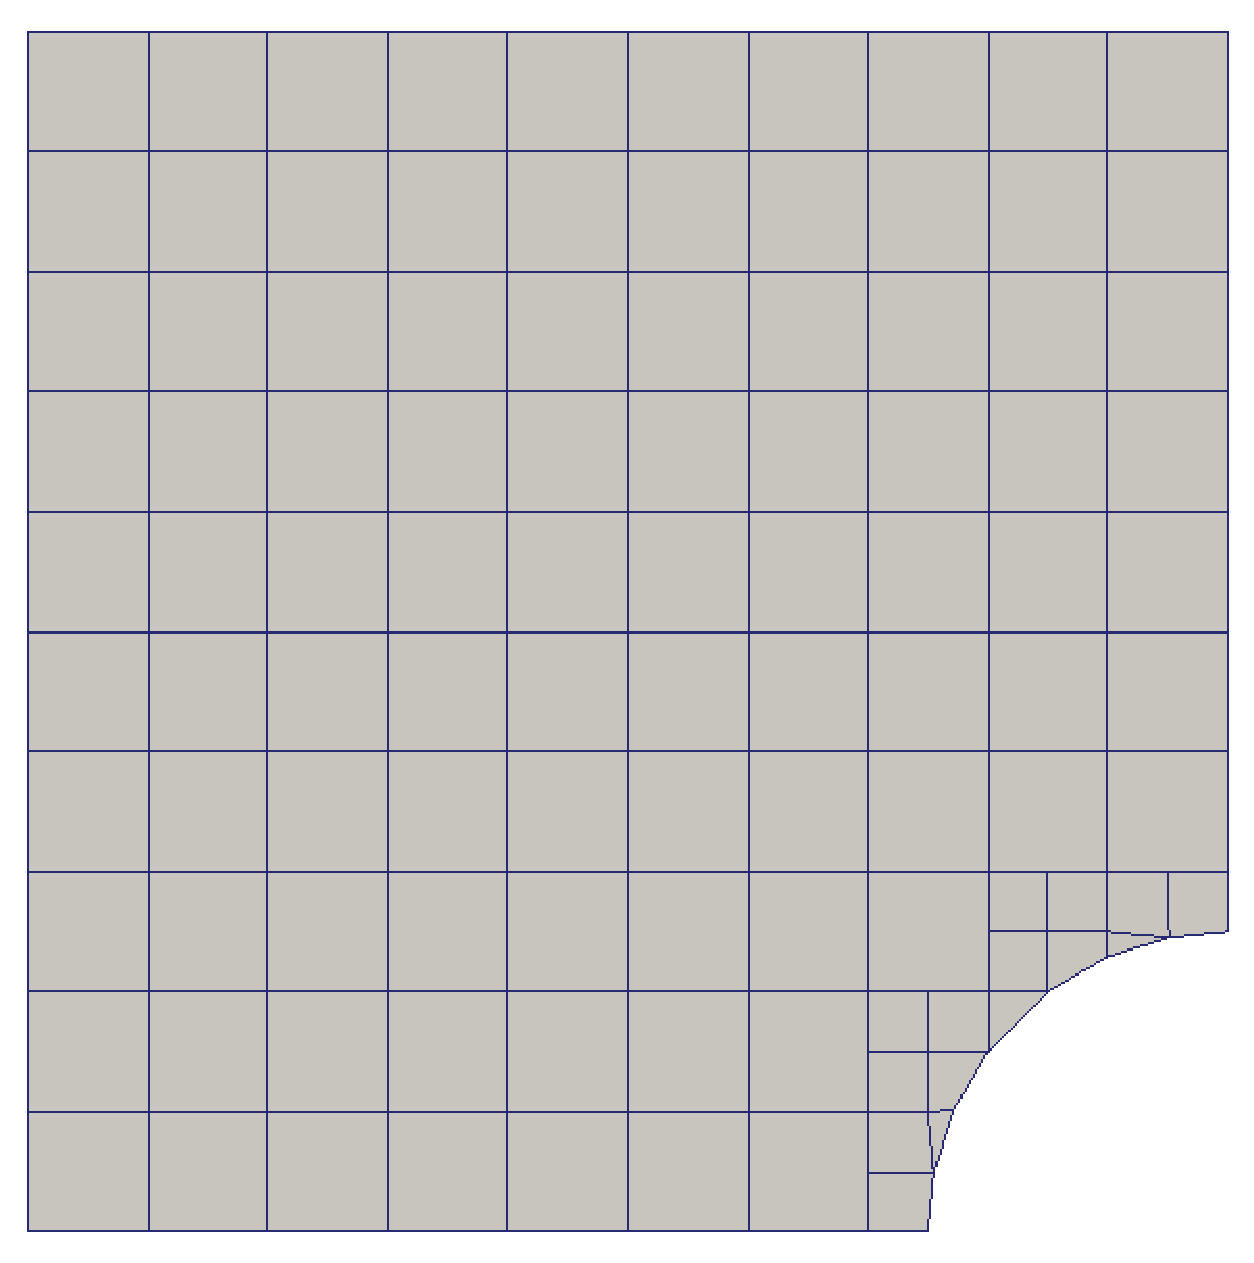
\includegraphics{quadtree/ex_images/ex_chole_mesh_262.eps}
    }
    \caption[Final mesh of infinite plate with a circular hole]{Final mesh of infinite plate with a circular hole}
    \label{qdt_fig:ex_chole_mesh_final}
\end{figure}
% 262 - 0.0112 (32-4/5-4)
% 290 - 0.0101 (64-4/5-4)
% 876 - 0.0036216 (128-4/8-4)
% 3280- 0.0010068 (256-4/15-4)
\paragraph{}
Mesh with different parameters are plotted in Fig.~\ref{qdt_fig:ex_chole_mesh_all} and the convergence study is plotted in Fig.~\ref{qdt_fig:ex_chole_mesh_conv}

\begin{figure}[H]
    \begin{subfigure}[b]{1\linewidth}
        \centering
        \scalebox{0.35}{
            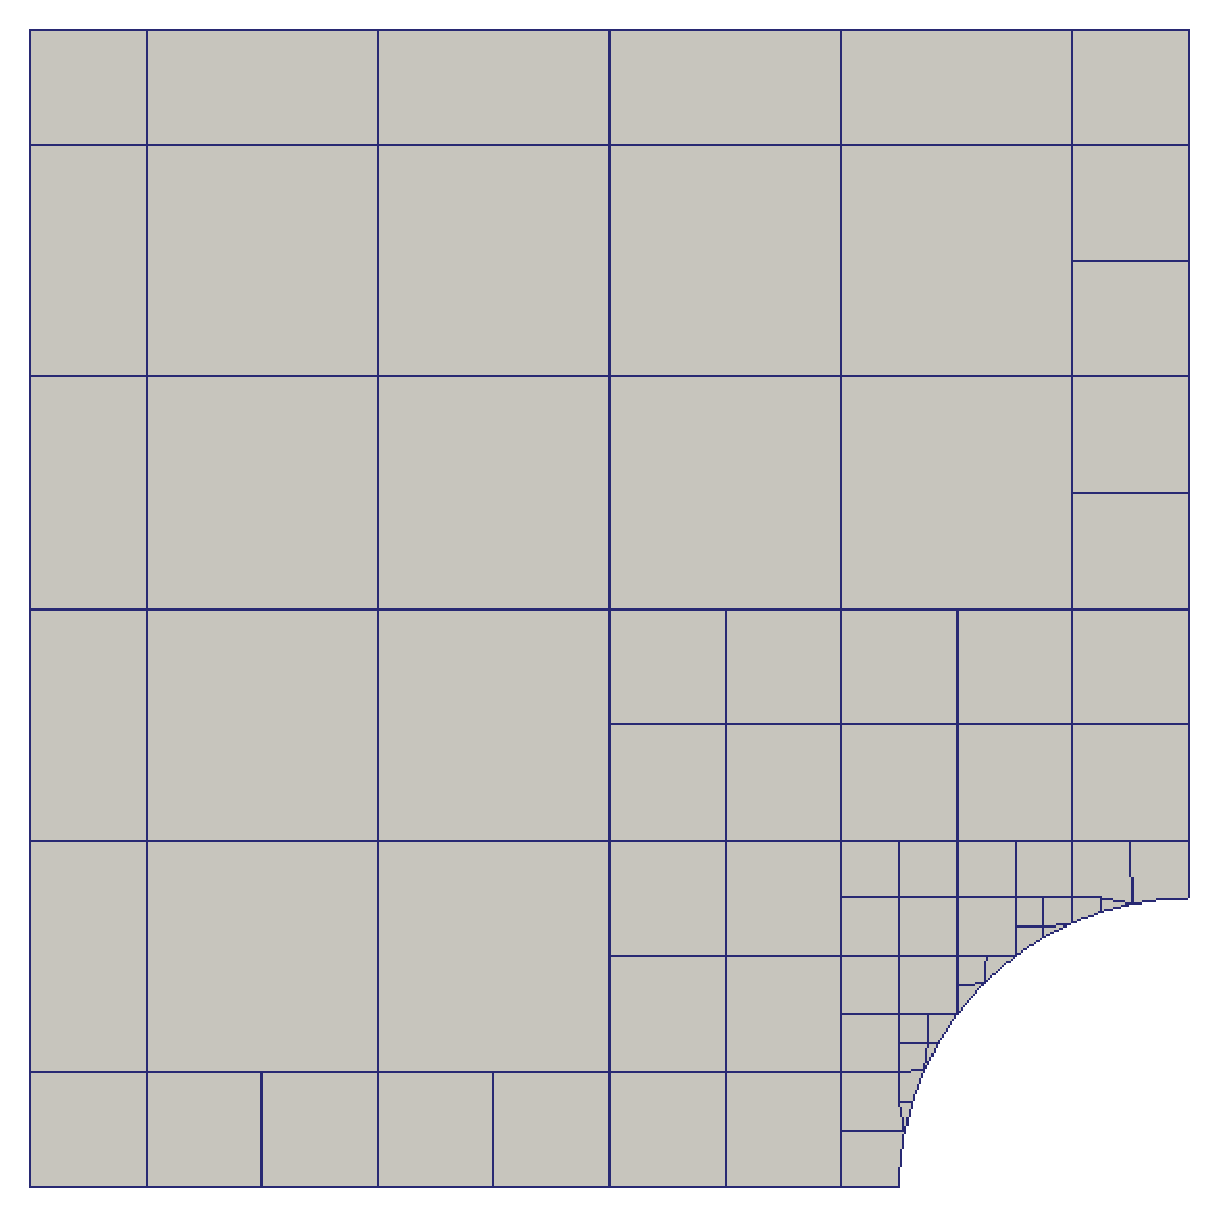
\includegraphics{quadtree/ex_images/qdt_chole_64_8.eps}
        }
        \caption{Mesh with $res=64$, $s_{max}=8$, 152 DOFs}
    \end{subfigure}
    \\
    \begin{subfigure}[b]{1\linewidth}
        \centering
        \scalebox{0.35}{
            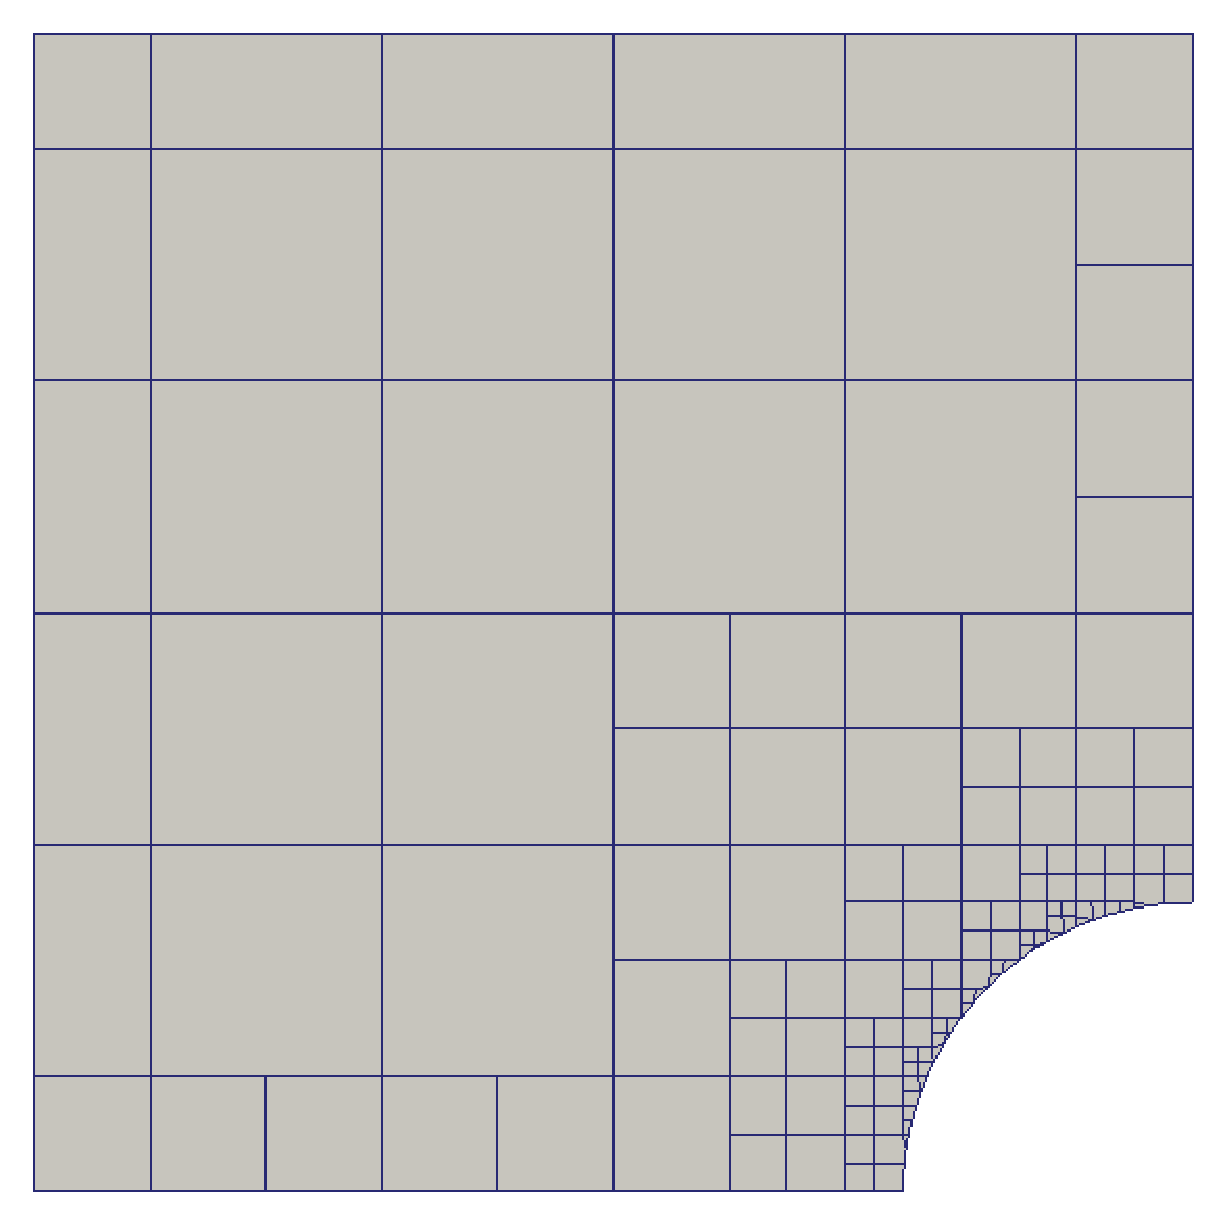
\includegraphics{quadtree/ex_images/qdt_chole_128_16.eps}
        }
        \caption{Mesh with $res=128$, $s_{max}=4$, 272 DOFs}
    \end{subfigure}
\end{figure}

\begin{figure}[H]\ContinuedFloat
    \begin{subfigure}[b]{1\linewidth}
        \centering
        \scalebox{0.35}{
            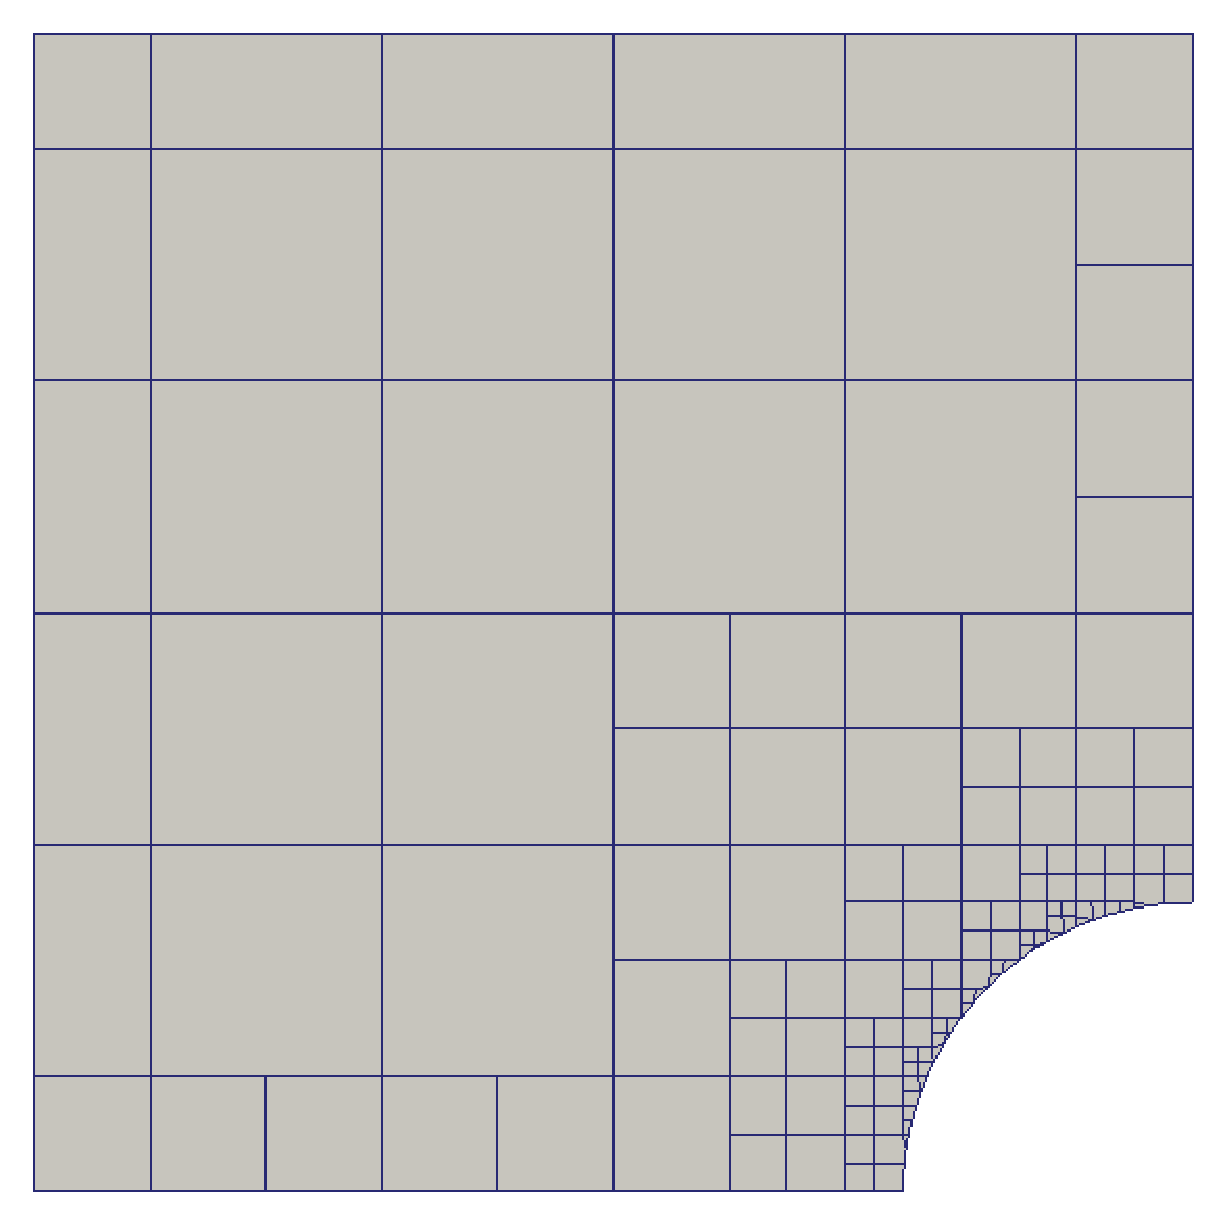
\includegraphics{quadtree/ex_images/qdt_chole_128_16.eps}
        }
        \caption{Mesh with $res=128$, $s_{max}=16$, 488 DOFs}
    \end{subfigure}
    \caption[Mesh of the infinite plate with a circular hole]{Mesh of infinite plate with a circular hole}
    \label{qdt_fig:ex_chole_mesh_all}
\end{figure}


\begin{figure}[H]
    \centering
    \scalebox{0.6}{
        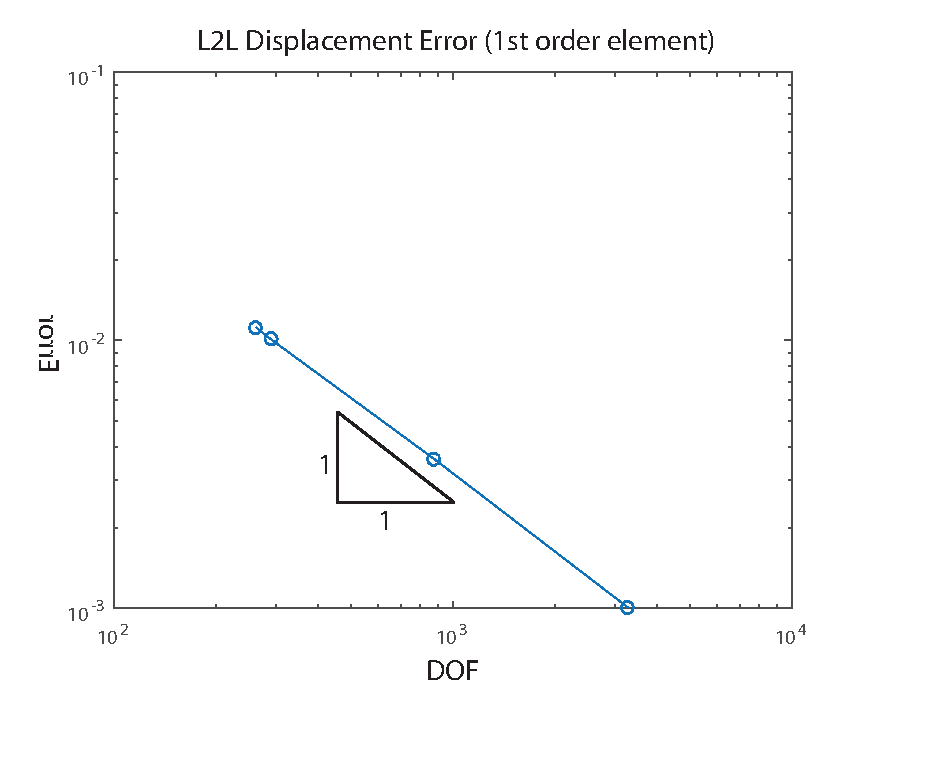
\includegraphics{quadtree/ex_images/ex_chole_conv.eps}
    }   
    \caption[Convergence of the infinite plate with a circular hole]{Convergence of the infinite plate with a circular hole}
    \label{qdt_fig:ex_chole_mesh_conv}
\end{figure}

\pagebreak
\subsection{Plane strain bracket}
\paragraph{}
In this example, a plane strain bracket with a downward uniform distributed load on the top is considered (see fig.~\ref{qdt_fig:ex_bracket_geo_bc}).
The material properties are: Young’s modulus $E = 2\times 10^5 N/m^2$ and Poisson’s ratio $\nu = 0.3$.
    \begin{figure}[H]
        \centering
        \begin{subfigure}[b]{1\linewidth}
            \centering
            \scalebox{1.5}{
                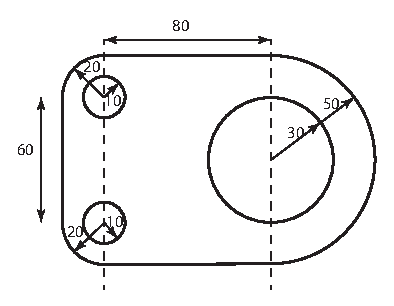
\includegraphics{quadtree/ex_images/ex_bracket_geo.eps}
            }
        \end{subfigure}
        \begin{subfigure}[b]{1\linewidth}
            \centering
            \scalebox{1.5}{
                
\includegraphics{quadtree/ex_images/ex_bracket_load.eps}
            }
        \end{subfigure}
        \caption{ Plane strain bracket: geometry and boundary conditions}
        \label{qdt_fig:ex_bracket_geo_bc}
    \end{figure}

\paragraph{}
A total strain energy of $282.927$ is determined by ANSYS with the mesh shown in fig.~\ref{qdt_fig:ex_bracket_ansys_mesh}
    \begin{figure}[H]
        \centering
        \scalebox{0.35}{
            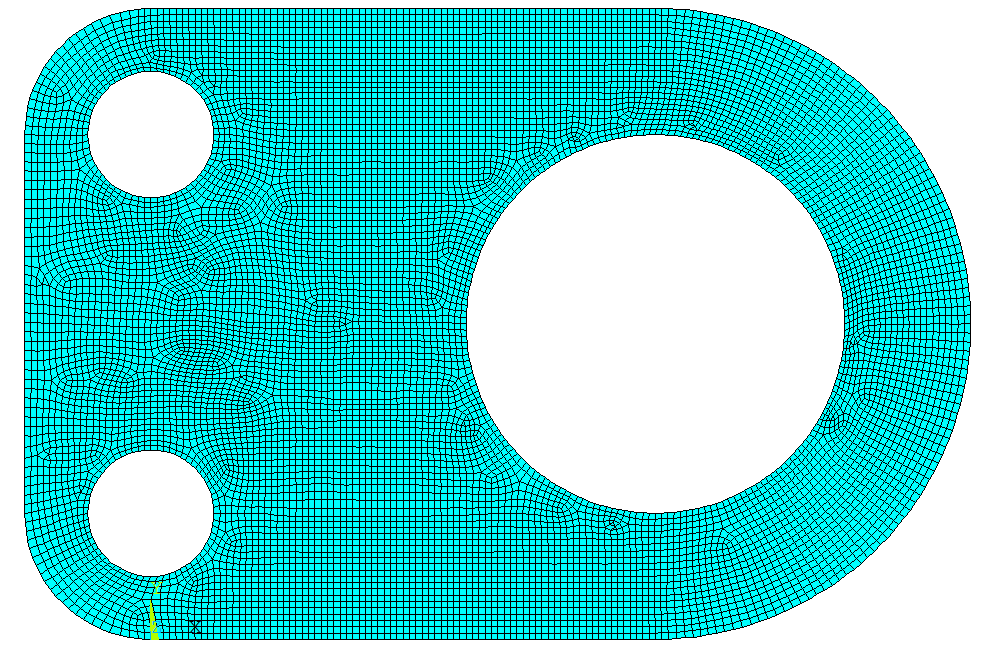
\includegraphics{quadtree/ex_images/ex_bracket_ansys_mesh_31002nodes.png}
        }
        \caption{ANSYS mesh for plane strain bracket (62004 DOF)}
        \label{qdt_fig:ex_bracket_ansys_mesh}
    \end{figure}

\paragraph{}
Drawing in AutoCAD will be divided into two parts: base and the holes as shown in fig.~\ref{qdt_fig:ex_bracket_cad}
    \begin{figure}[H]
        \centering
        \begin{subfigure}[b]{1\linewidth}
            \centering
            \scalebox{0.4}{
                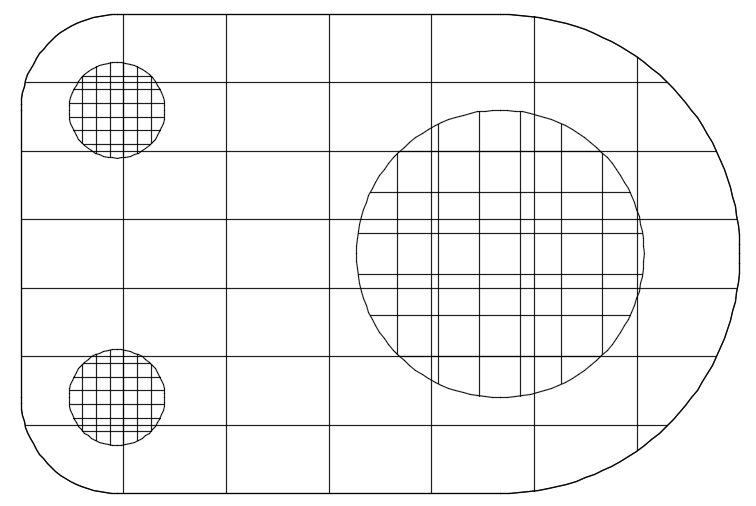
\includegraphics{quadtree/ex_images/ex_bracket_cad_full.png}
            }
            \caption{All}
        \end{subfigure}
        \begin{subfigure}[b]{0.4\linewidth}
            \scalebox{0.2}{
                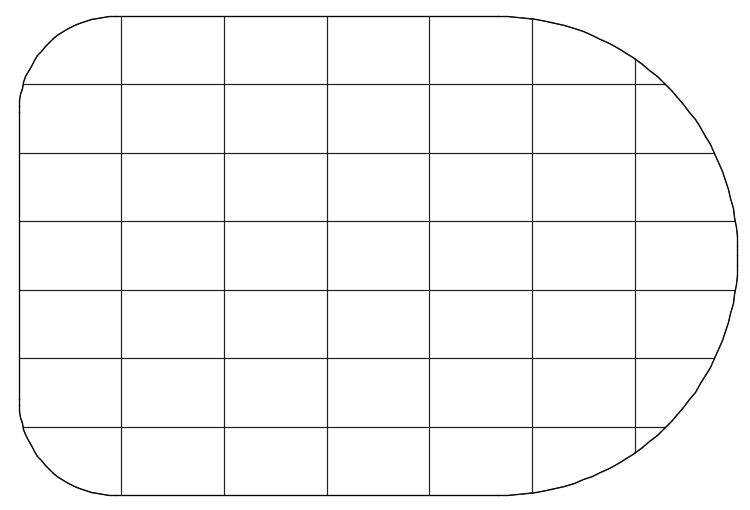
\includegraphics{quadtree/ex_images/ex_bracket_cad_base.png}
            }
            \caption{Base}
        \end{subfigure}
        \begin{subfigure}[b]{0.4\linewidth}
            \scalebox{0.2}{
                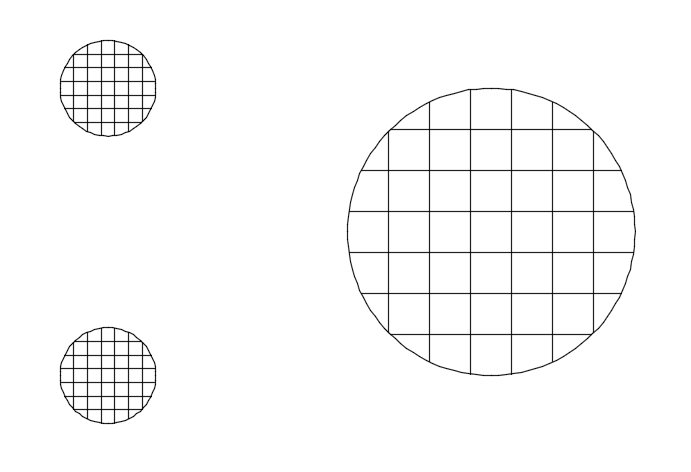
\includegraphics{quadtree/ex_images/ex_bracket_cad_holes.png}
            }
            \caption{Holes}
        \end{subfigure}
        \caption{CAD drawing of plane strain bracket}
        \label{qdt_fig:ex_bracket_cad}
    \end{figure}
% fig- 64,32/8,3
Generated background mesh, coloring and the final result with $res=32$, $s_{max}=4$ and $s_{min}=1$ are shown in fig.~\ref{qdt_fig:ex_chole_background_mesh}, fig.~\ref{qdt_fig:ex_chole_mesh_coloring} and fig.~\ref{qdt_fig:ex_chole_mesh_final}.
\begin{figure}
    \centering
    \scalebox{0.4}{
        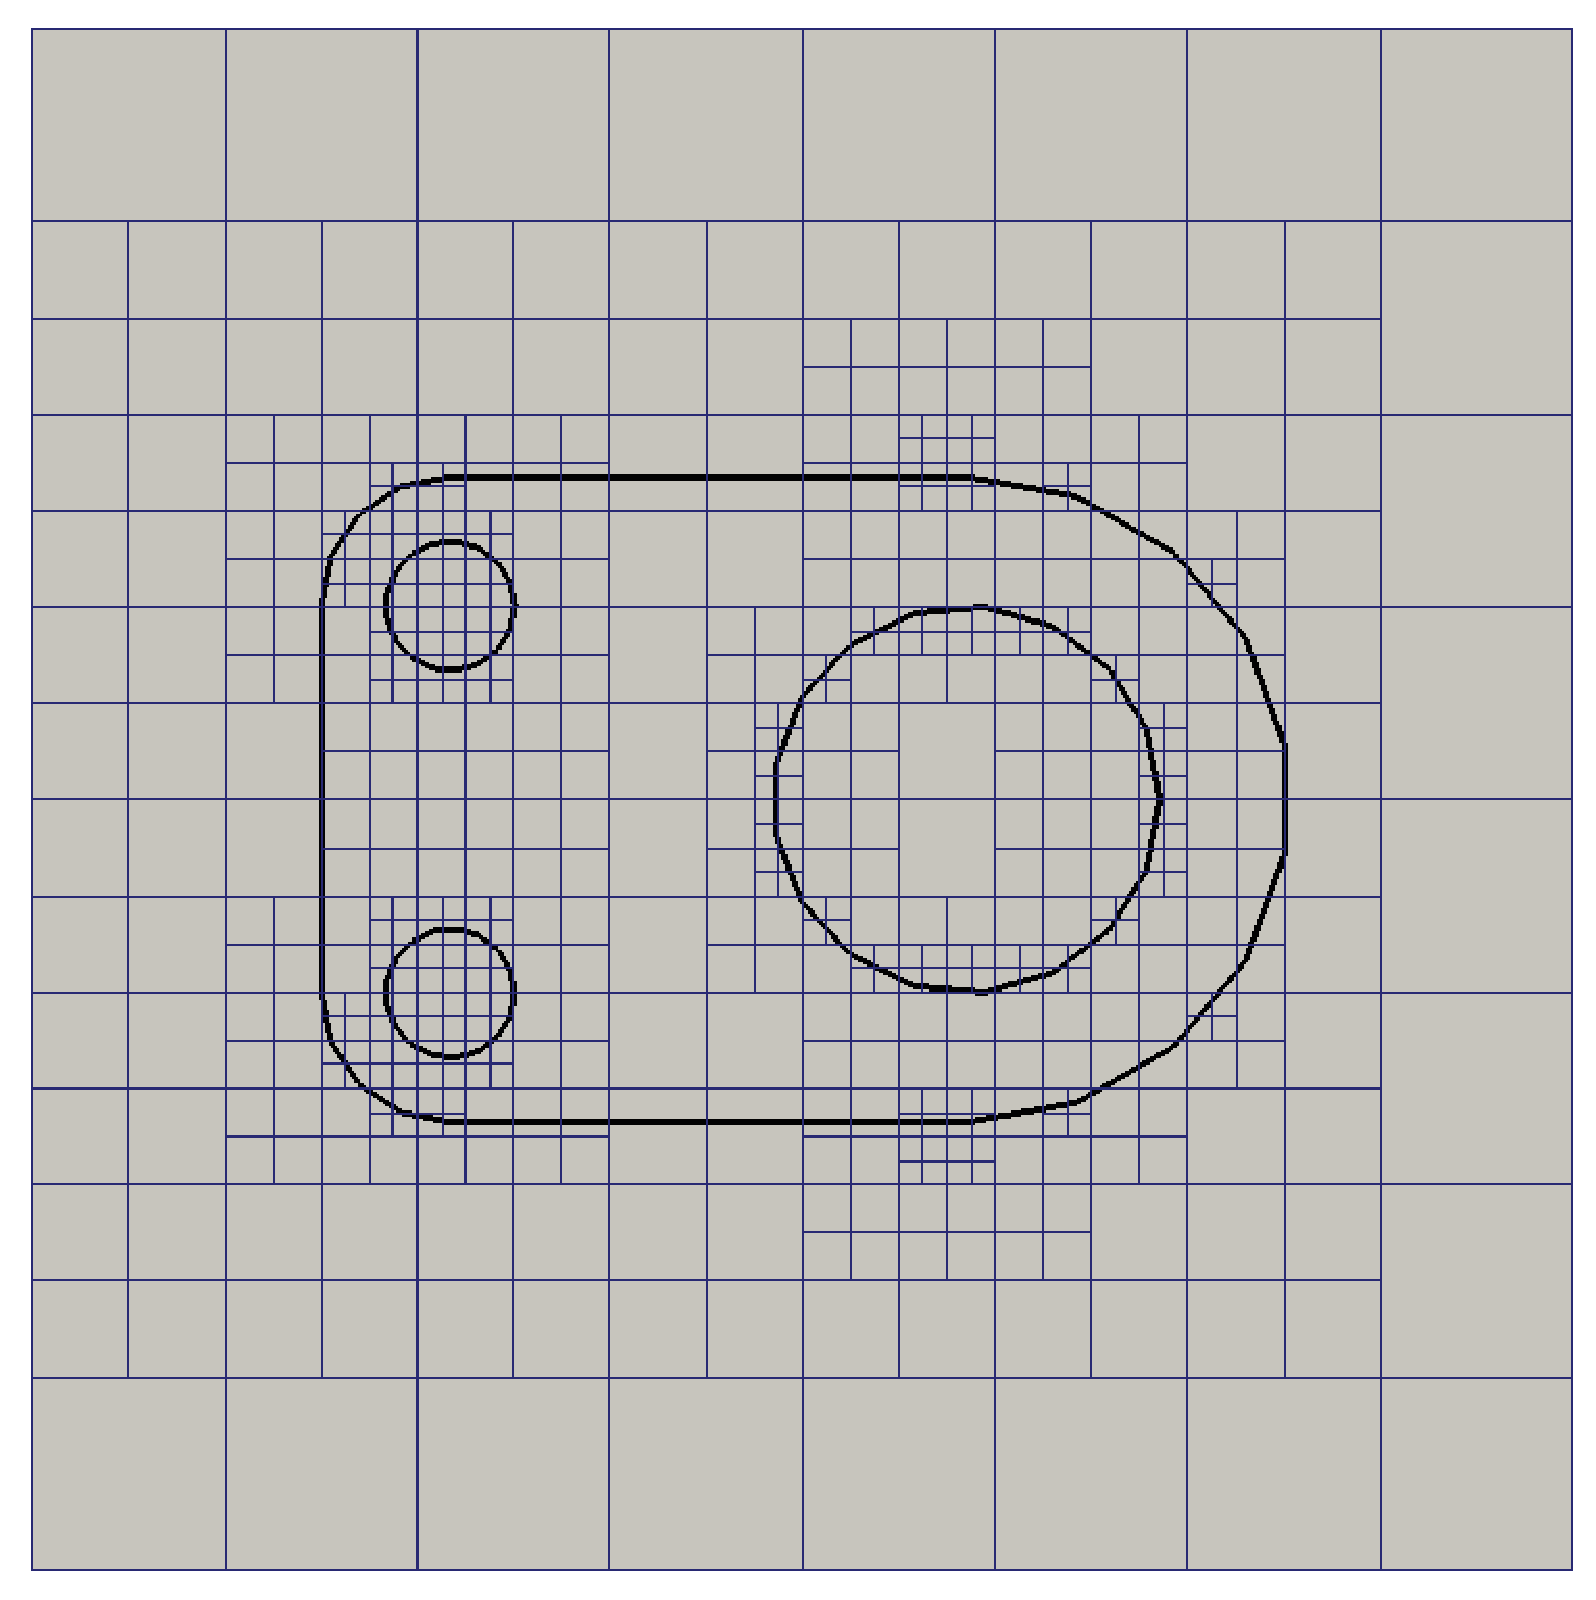
\includegraphics{quadtree/ex_images/ex_bracket_background.eps}
    }
    \caption[Background mesh of the bracket]{Background mesh of the bracket : Bold lines represents the input geometry}
    \label{qdt_fig:ex_chole_background_mesh}
\end{figure}

\begin{figure}
    \centering
    \scalebox{0.4}{
        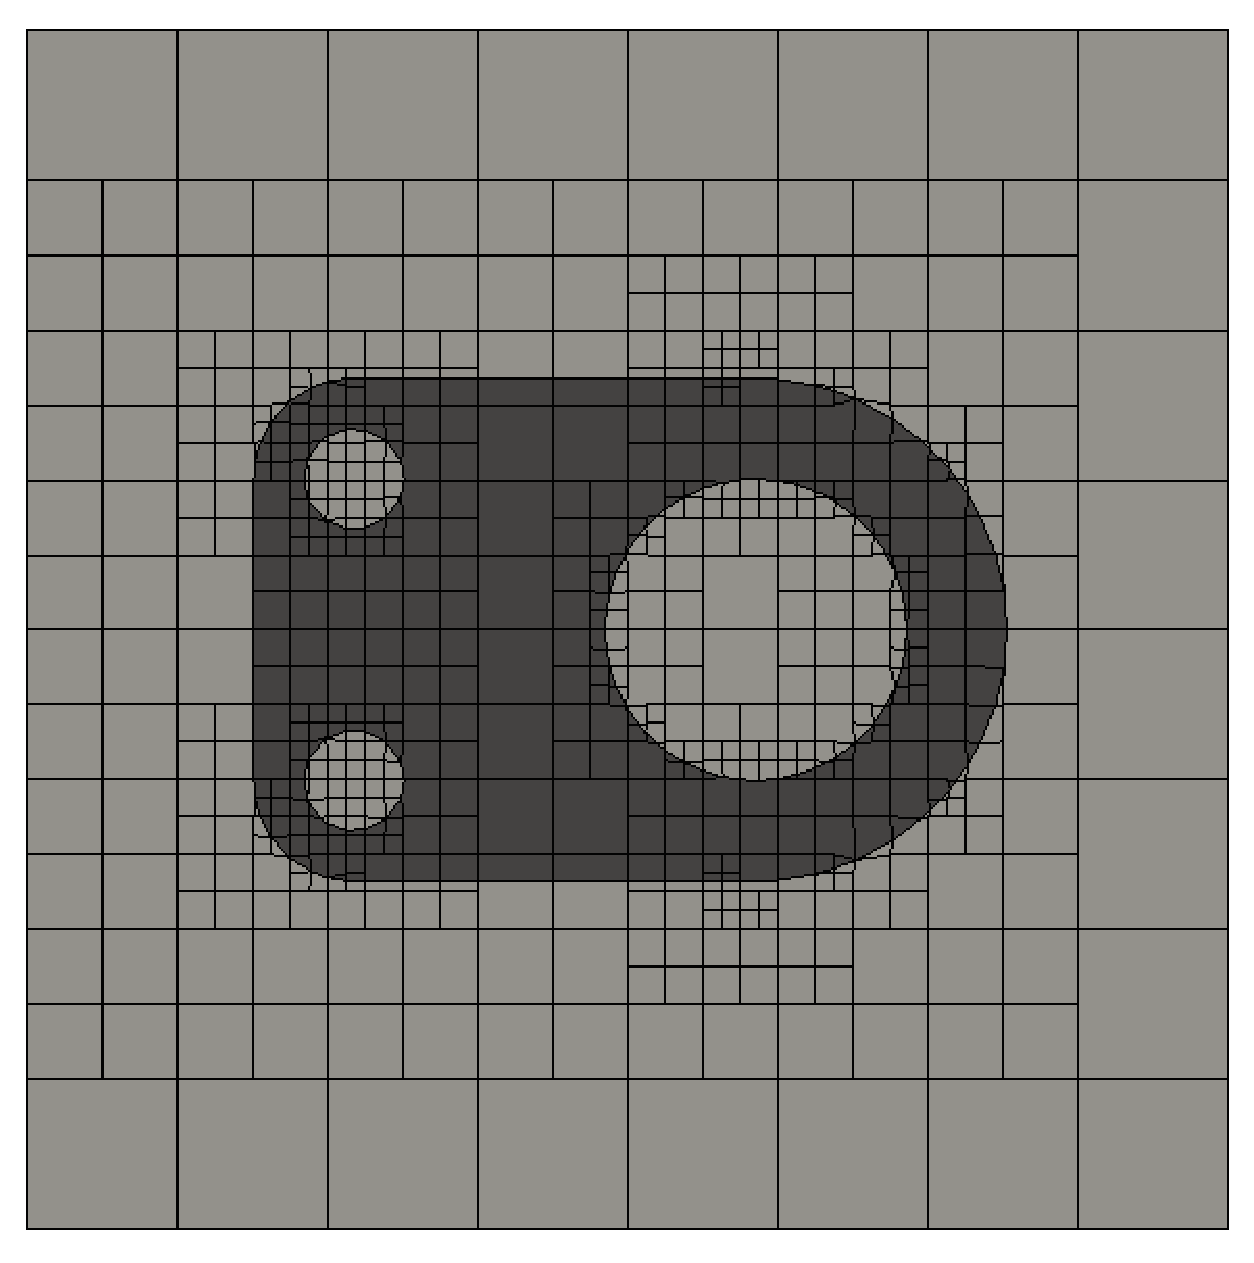
\includegraphics{quadtree/ex_images/ex_bracket_colored.eps}
    }
    \caption[Mesh coloring of the bracket]{Mesh coloring of the bracket : Grey area represents the bracket}
    \label{qdt_fig:ex_chole_mesh_coloring}
\end{figure}

\begin{figure}
    \centering
    \scalebox{0.3}{
        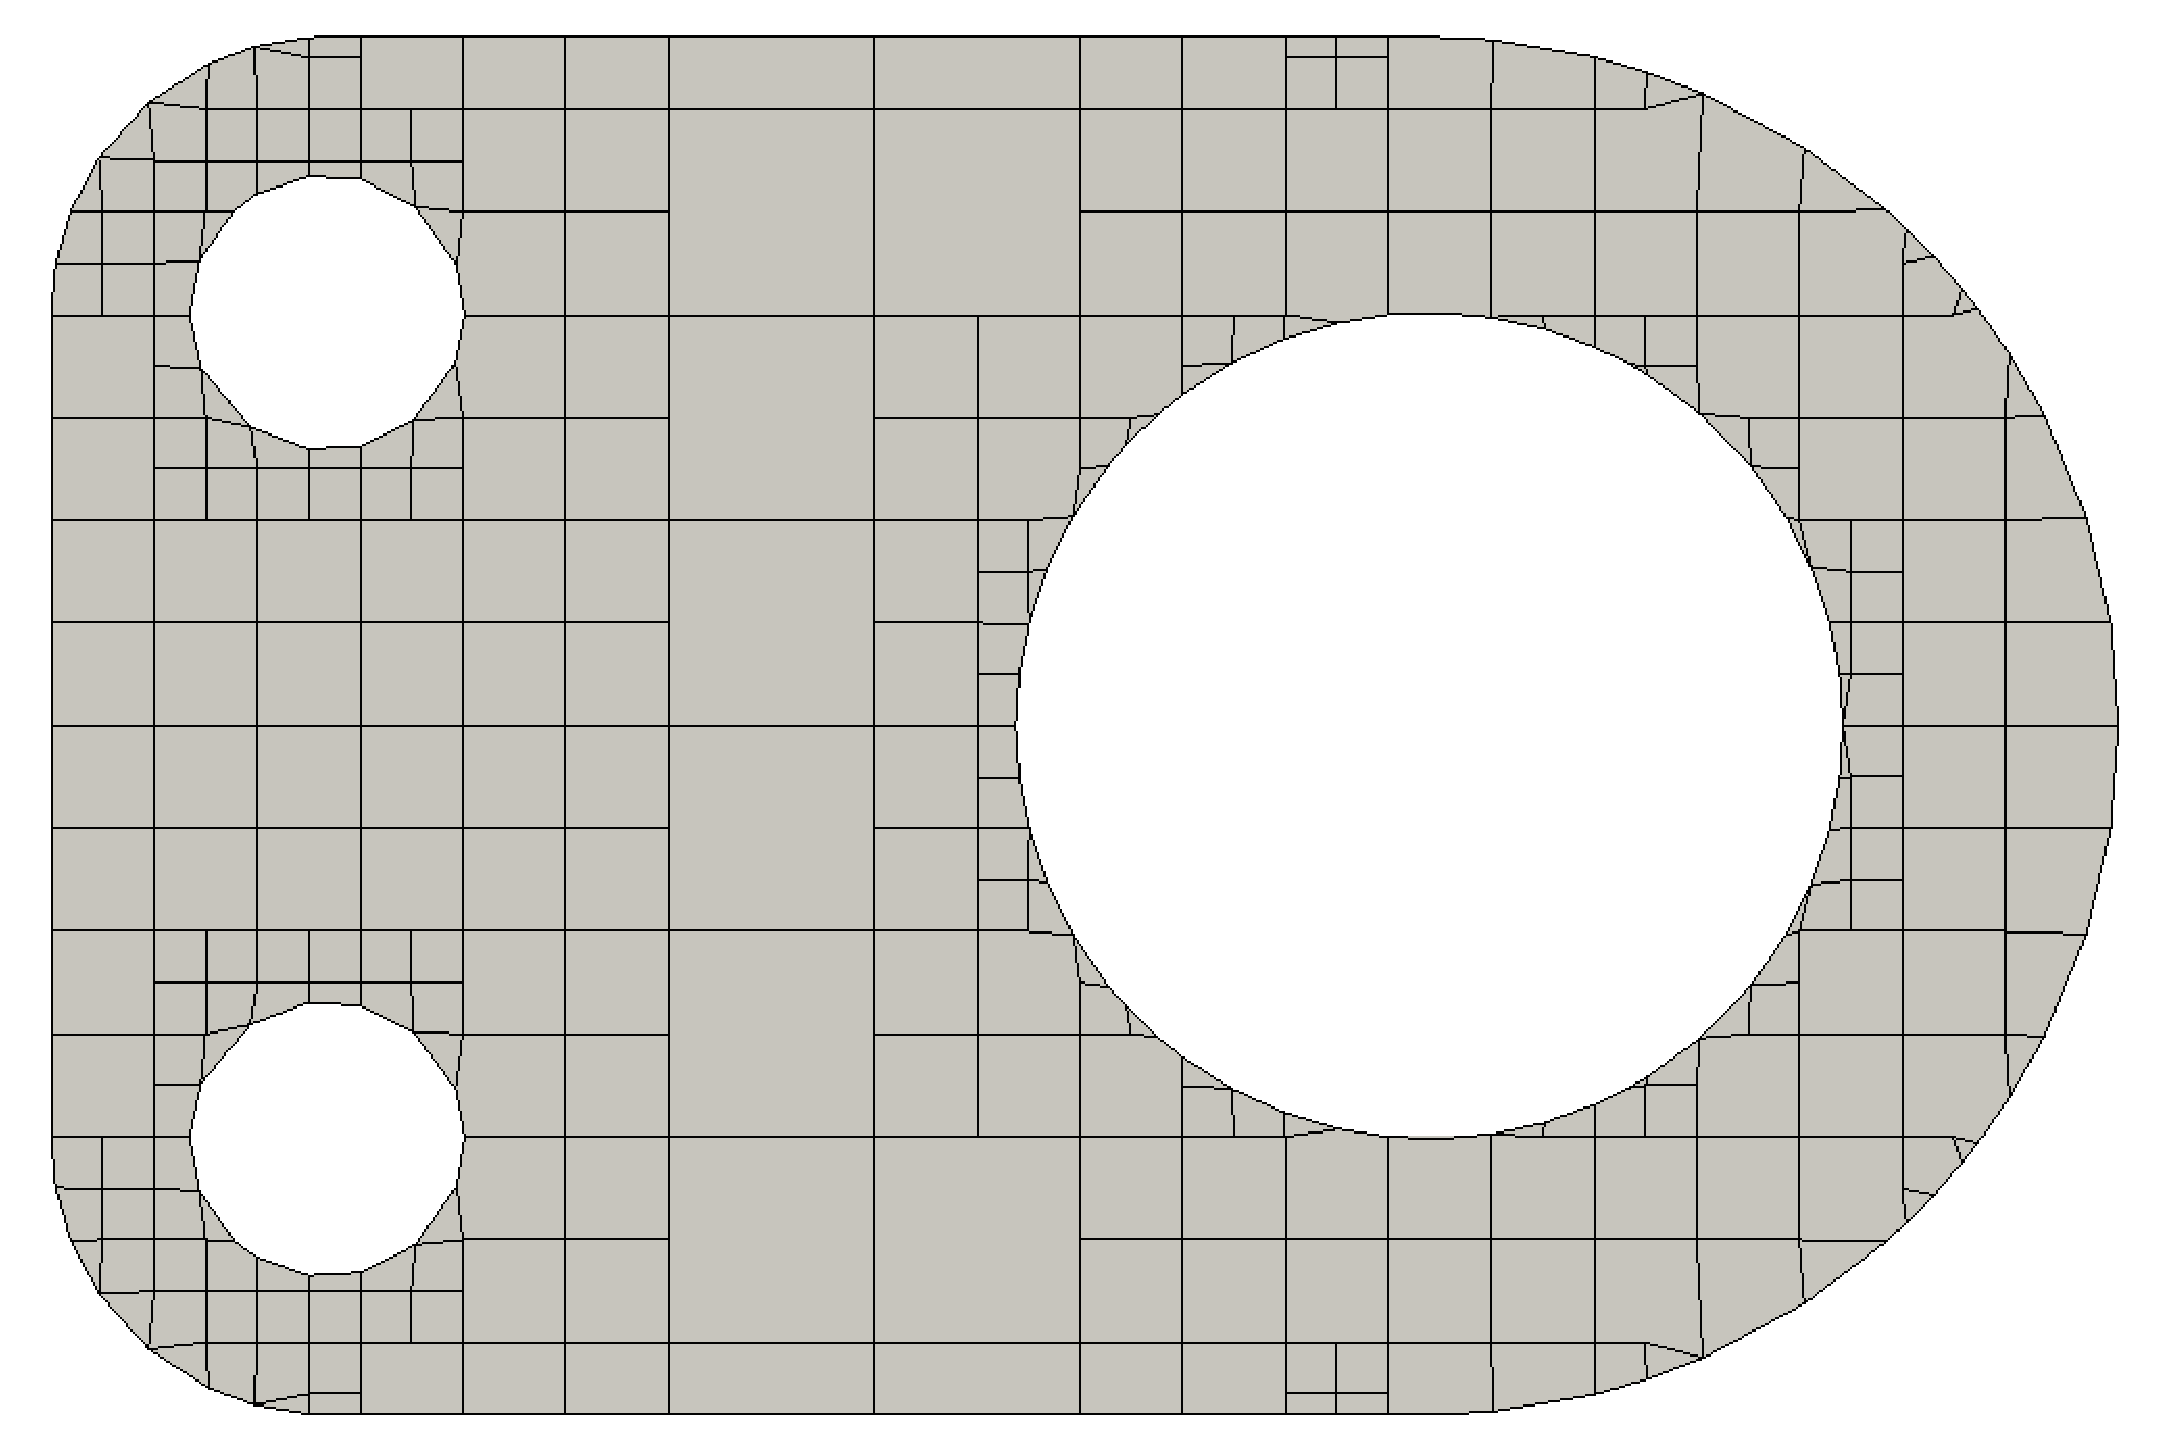
\includegraphics{quadtree/ex_images/ex_bracket_final.eps}
    }
    \caption[Final mesh of the bracket]{Final mesh of the bracket}
    \label{qdt_fig:ex_chole_mesh_final}
\end{figure}
% -1 - 282.927
% 382*2  - 274.5638 (32-4/8-3)
% 950*2  - 280.1255 (64-4/8-3)
% 2110*2 - 281.0799 (128-4/15-4)
% 4414*2 - 282.0363 (256-4/15-4)
Mesh with different parameters are plotted in fig.~\ref{qdt_fig:ex_bracket_mesh_all} and the convergence study is plotted in fig.~\ref{qdt_fig:ex_bracket_mesh_conv}

\begin{figure}[H]
    \begin{subfigure}[b]{1\linewidth}
        \centering
        \scalebox{0.4}{
            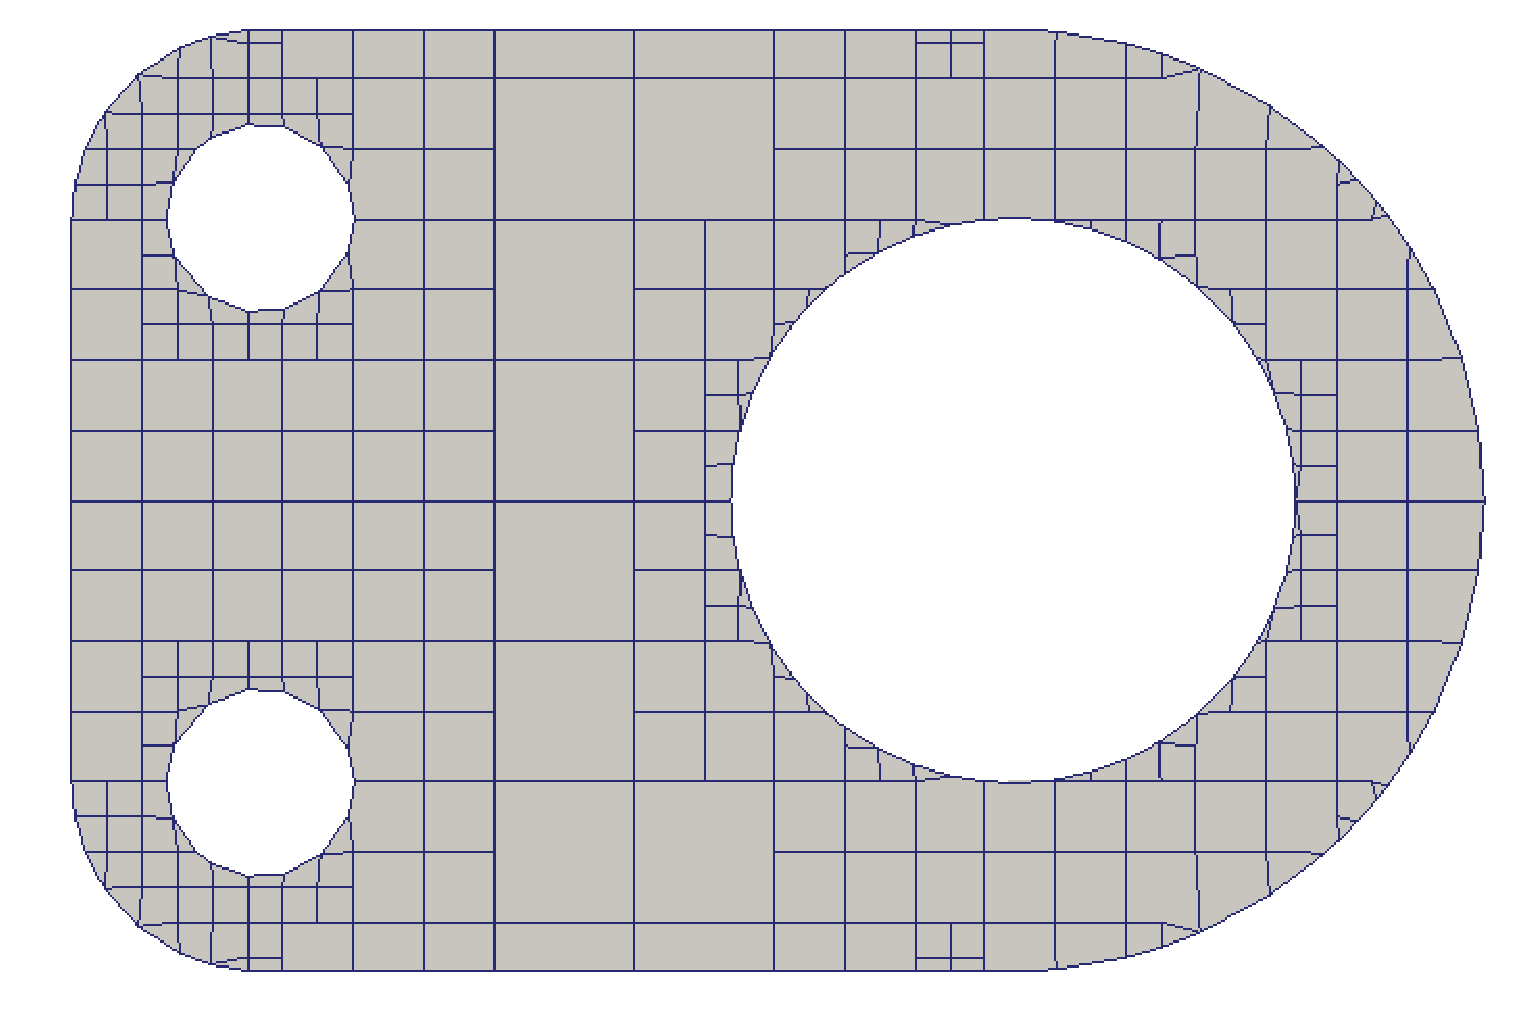
\includegraphics{quadtree/ex_images/ex_bracket_mesh_64_4.eps}
        }
        \caption{Mesh with $res=64$, $s_{max}=4$, 1656 DOFs}
    \end{subfigure}
    \\
    \begin{subfigure}[b]{1\linewidth}
        \centering
        \scalebox{0.4}{
            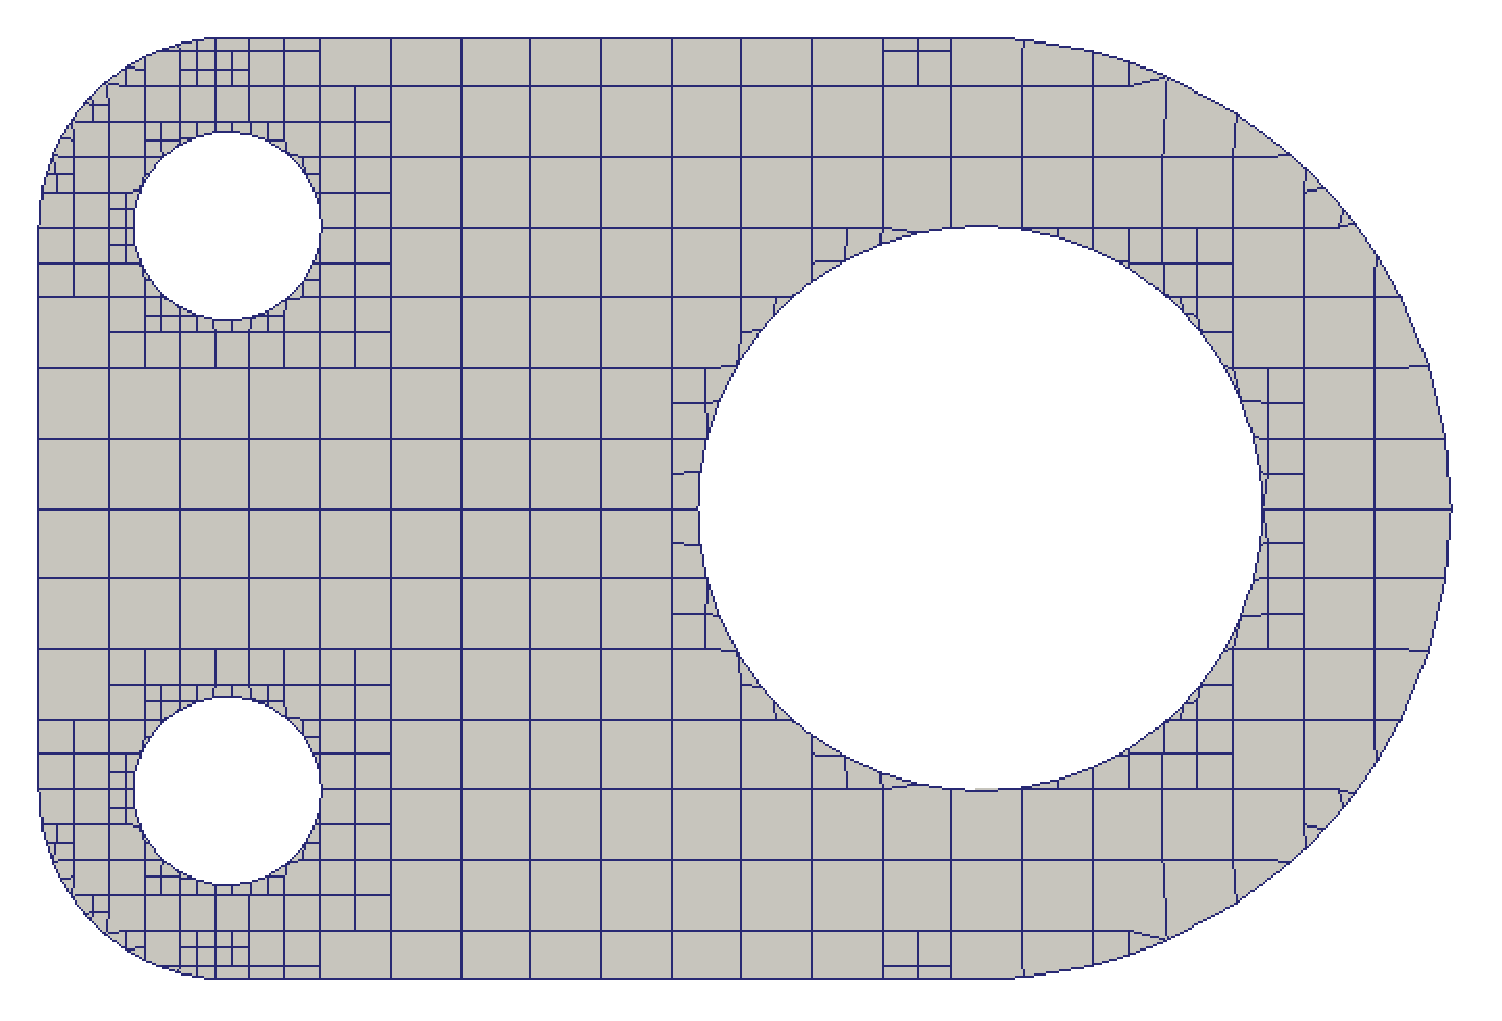
\includegraphics{quadtree/ex_images/ex_bracket_mesh_128_4.eps}
        }
        \caption{Mesh with $res=128$, $s_{max}=4$, 2548 DOFs}
    \end{subfigure}
\end{figure}

\begin{figure}[H]\ContinuedFloat
    \begin{subfigure}[b]{1\linewidth}
        \centering
        \scalebox{0.5}{
            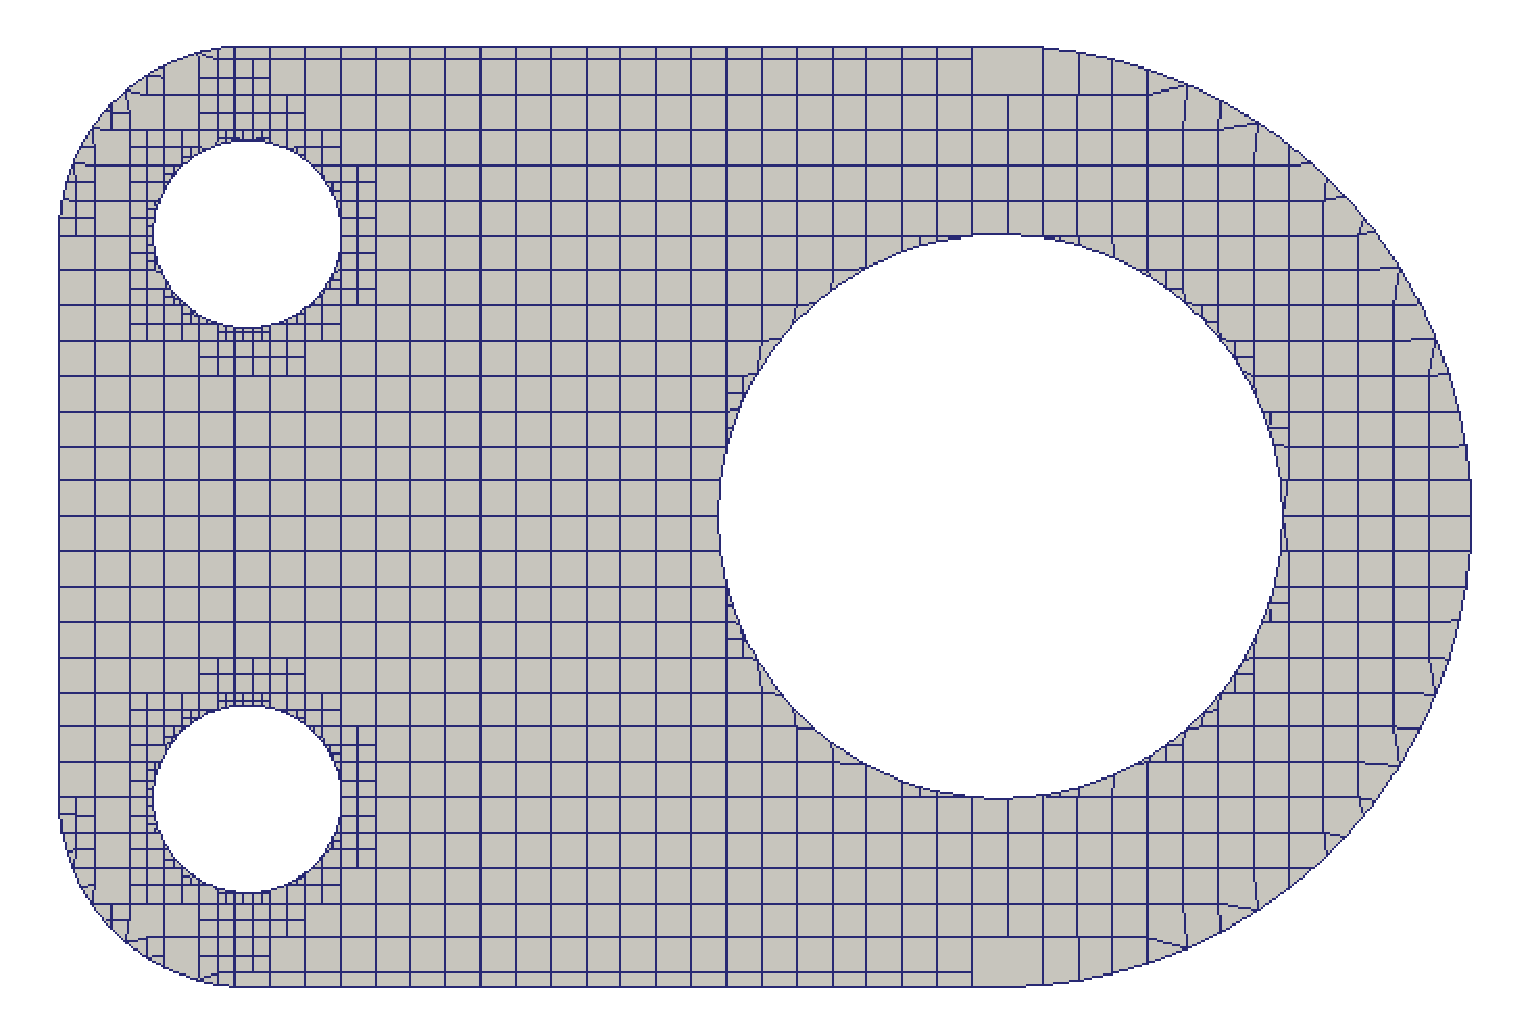
\includegraphics{quadtree/ex_images/ex_bracket_mesh_256_4.eps}
        }
        \caption{Mesh with $res=256$, $s_{max}=4$, 5464 DOFs}
    \end{subfigure}
    \caption[Mesh of the plane strain bracket]{Mesh of the plane strain bracket}
    \label{qdt_fig:ex_bracket_mesh_all}
\end{figure}

\begin{figure}[H]
    \centering
    \scalebox{0.75}{
        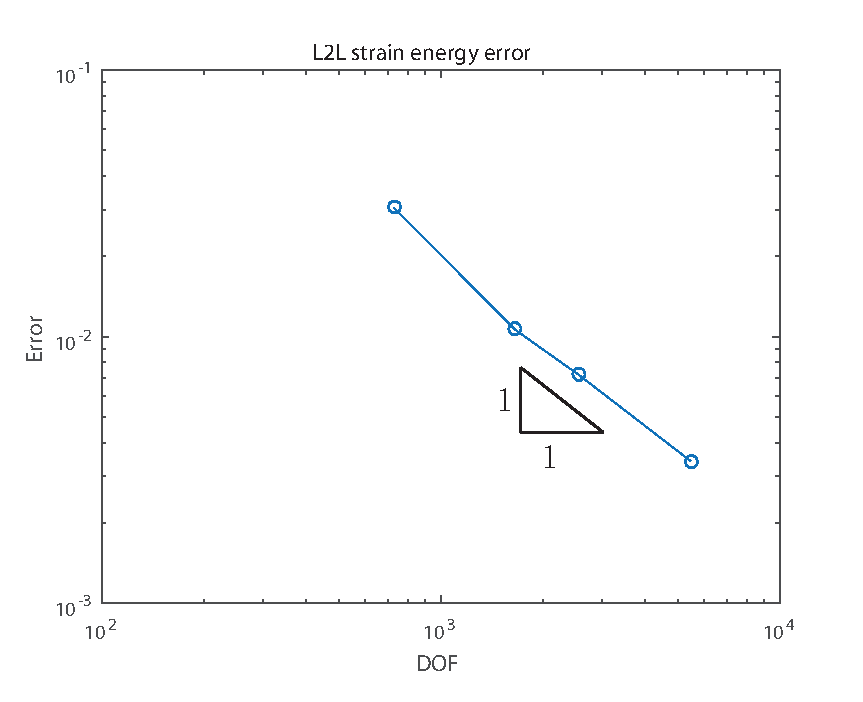
\includegraphics{quadtree/ex_images/ex_bracket_conv.eps}
    }   
    \caption[Convergence of the plane strain bracket]{Convergence of the plane strain bracket}
    \label{qdt_fig:ex_bracket_mesh_conv}
\end{figure}


\paragraph{}
Fig.~\ref{qdt_fig:bracket_stress_contour} shows the von Mises equivalent stress for the plane strain bracket.
From Fig.~\ref{qdt_fig:bracket_stress_contour}, it can be observed that the results from the present approach qualitatively match with the FE solution.
\begin{figure}[h!]
    \begin{subfigure}[b]{1\linewidth}
        \centering
        \scalebox{0.4}{
            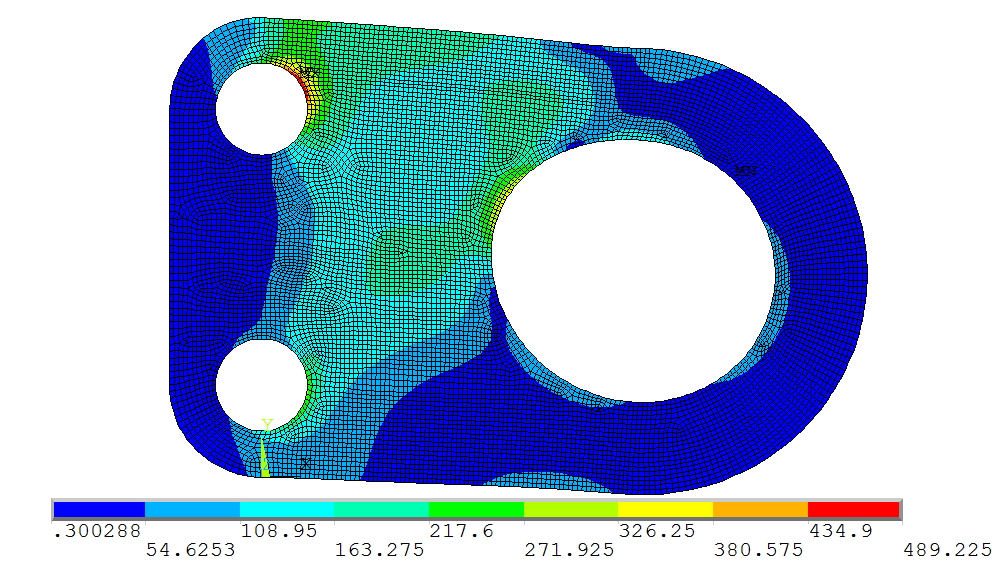
\includegraphics{quadtree/ex_images/ex_bracket_ansys_vmstr.png}
        }
        \caption{FEM}
    \end{subfigure}
    \begin{subfigure}[b]{1\linewidth}
        \centering
        \scalebox{0.4}{
            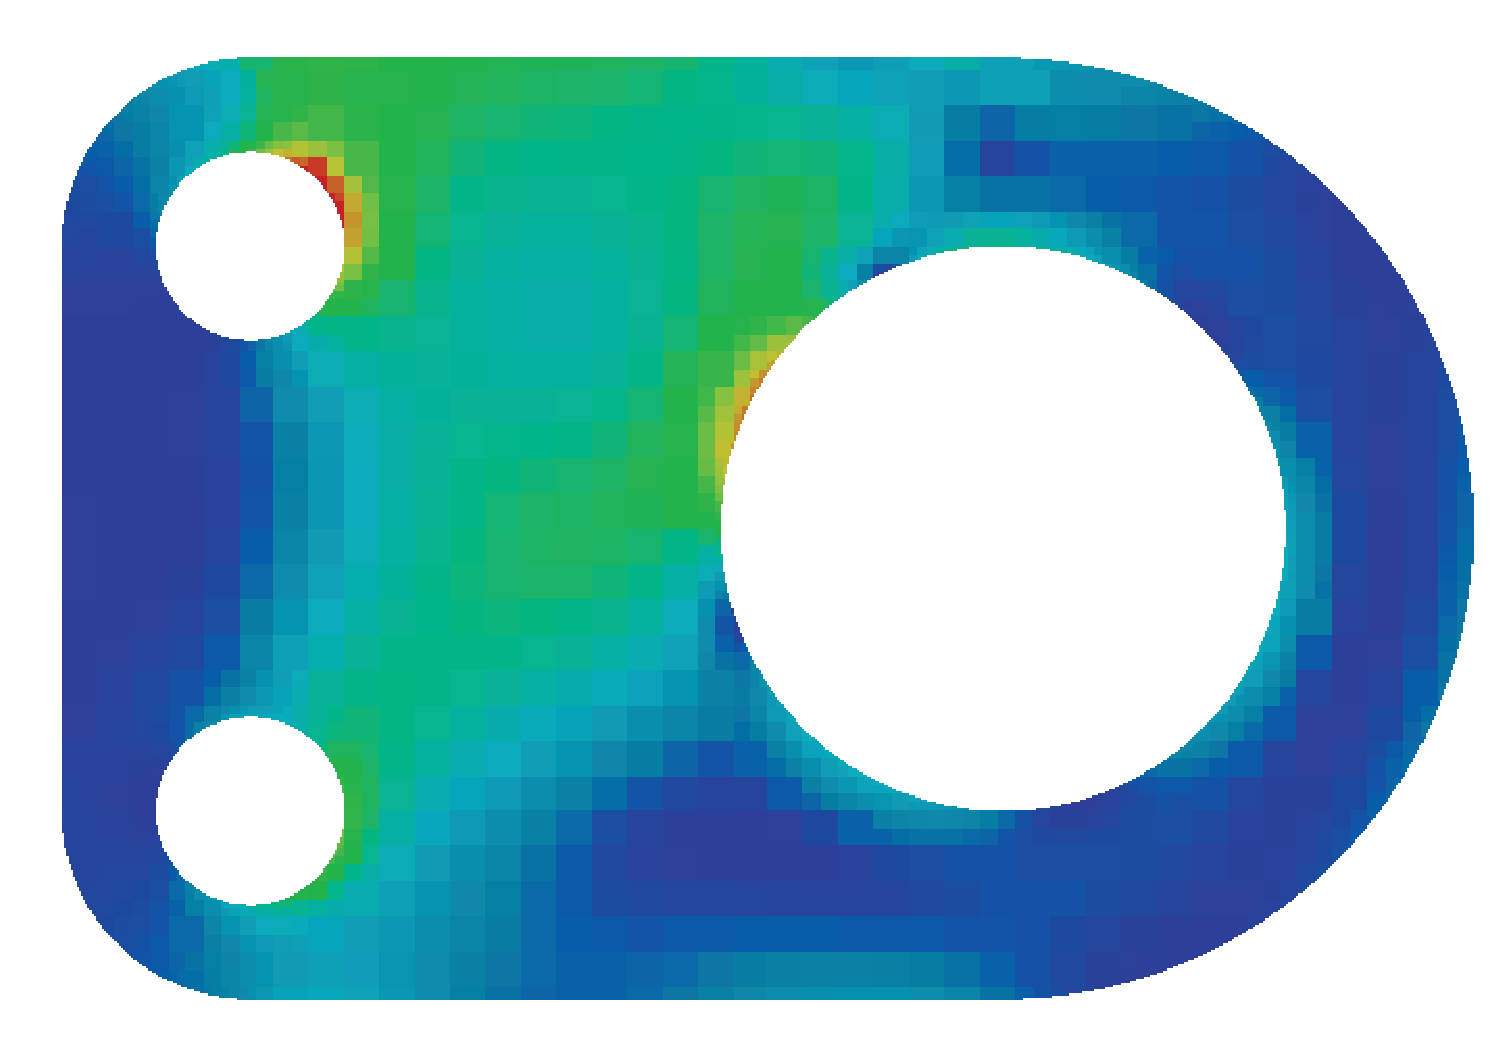
\includegraphics{quadtree/ex_images/ex_bracket_strcontour.eps}
        }
        \caption{Quadtree SBFEM}
    \end{subfigure}

    \caption{Von Mises equivalent stress contours for plane strain bracket}
    \label{qdt_fig:bracket_stress_contour}
\end{figure}
% \input{quadtree/ex_dam.tex}
\subsection{Buildings on the ground}

\begin{figure}
    \centering
    \scalebox{0.5}{
        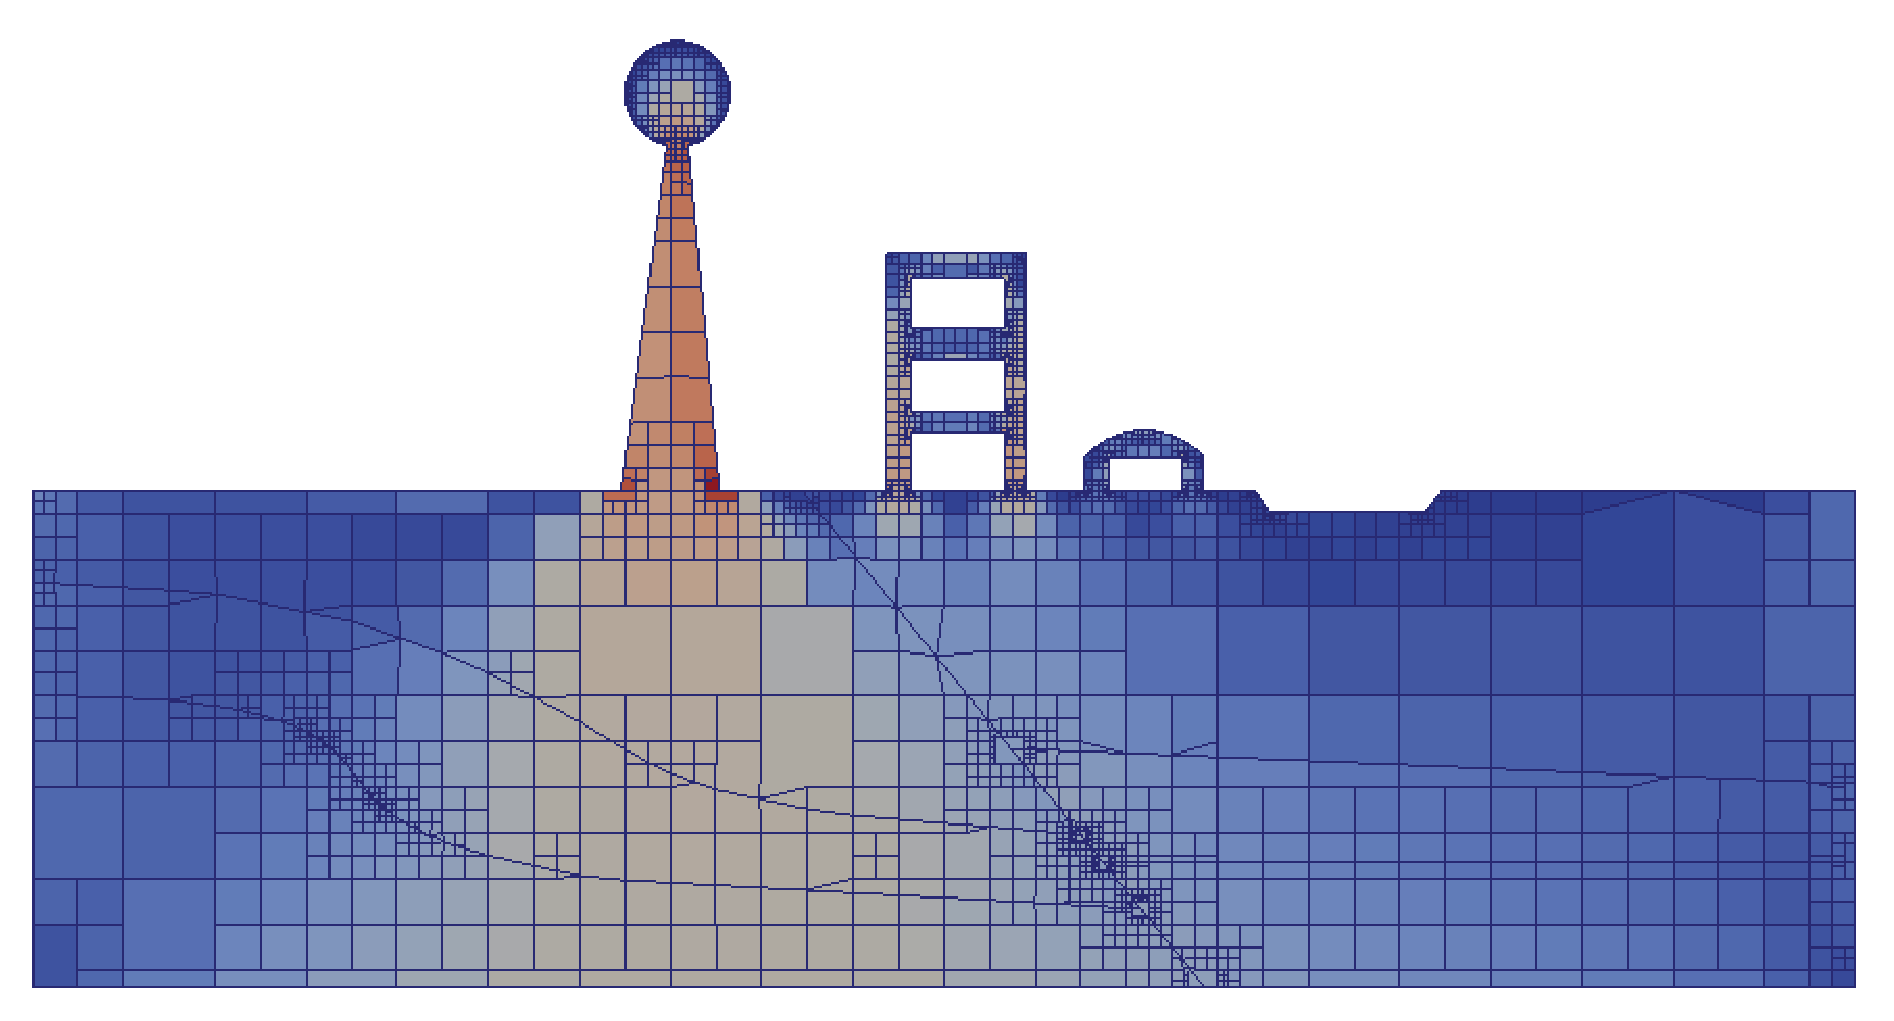
\includegraphics{quadtree/ex_images/ex_building_stress.eps}
    }
    \caption{Von-mises stress contour for the buidlings on the ground}
    % \label{qdt_fig:ex_cantilever_beam_background_mesh}
\end{figure}

\subsection{Other meshes}
\begin{figure}[h!]
    \begin{subfigure}[b]{1\linewidth}
        \centering
        \scalebox{0.3}{
            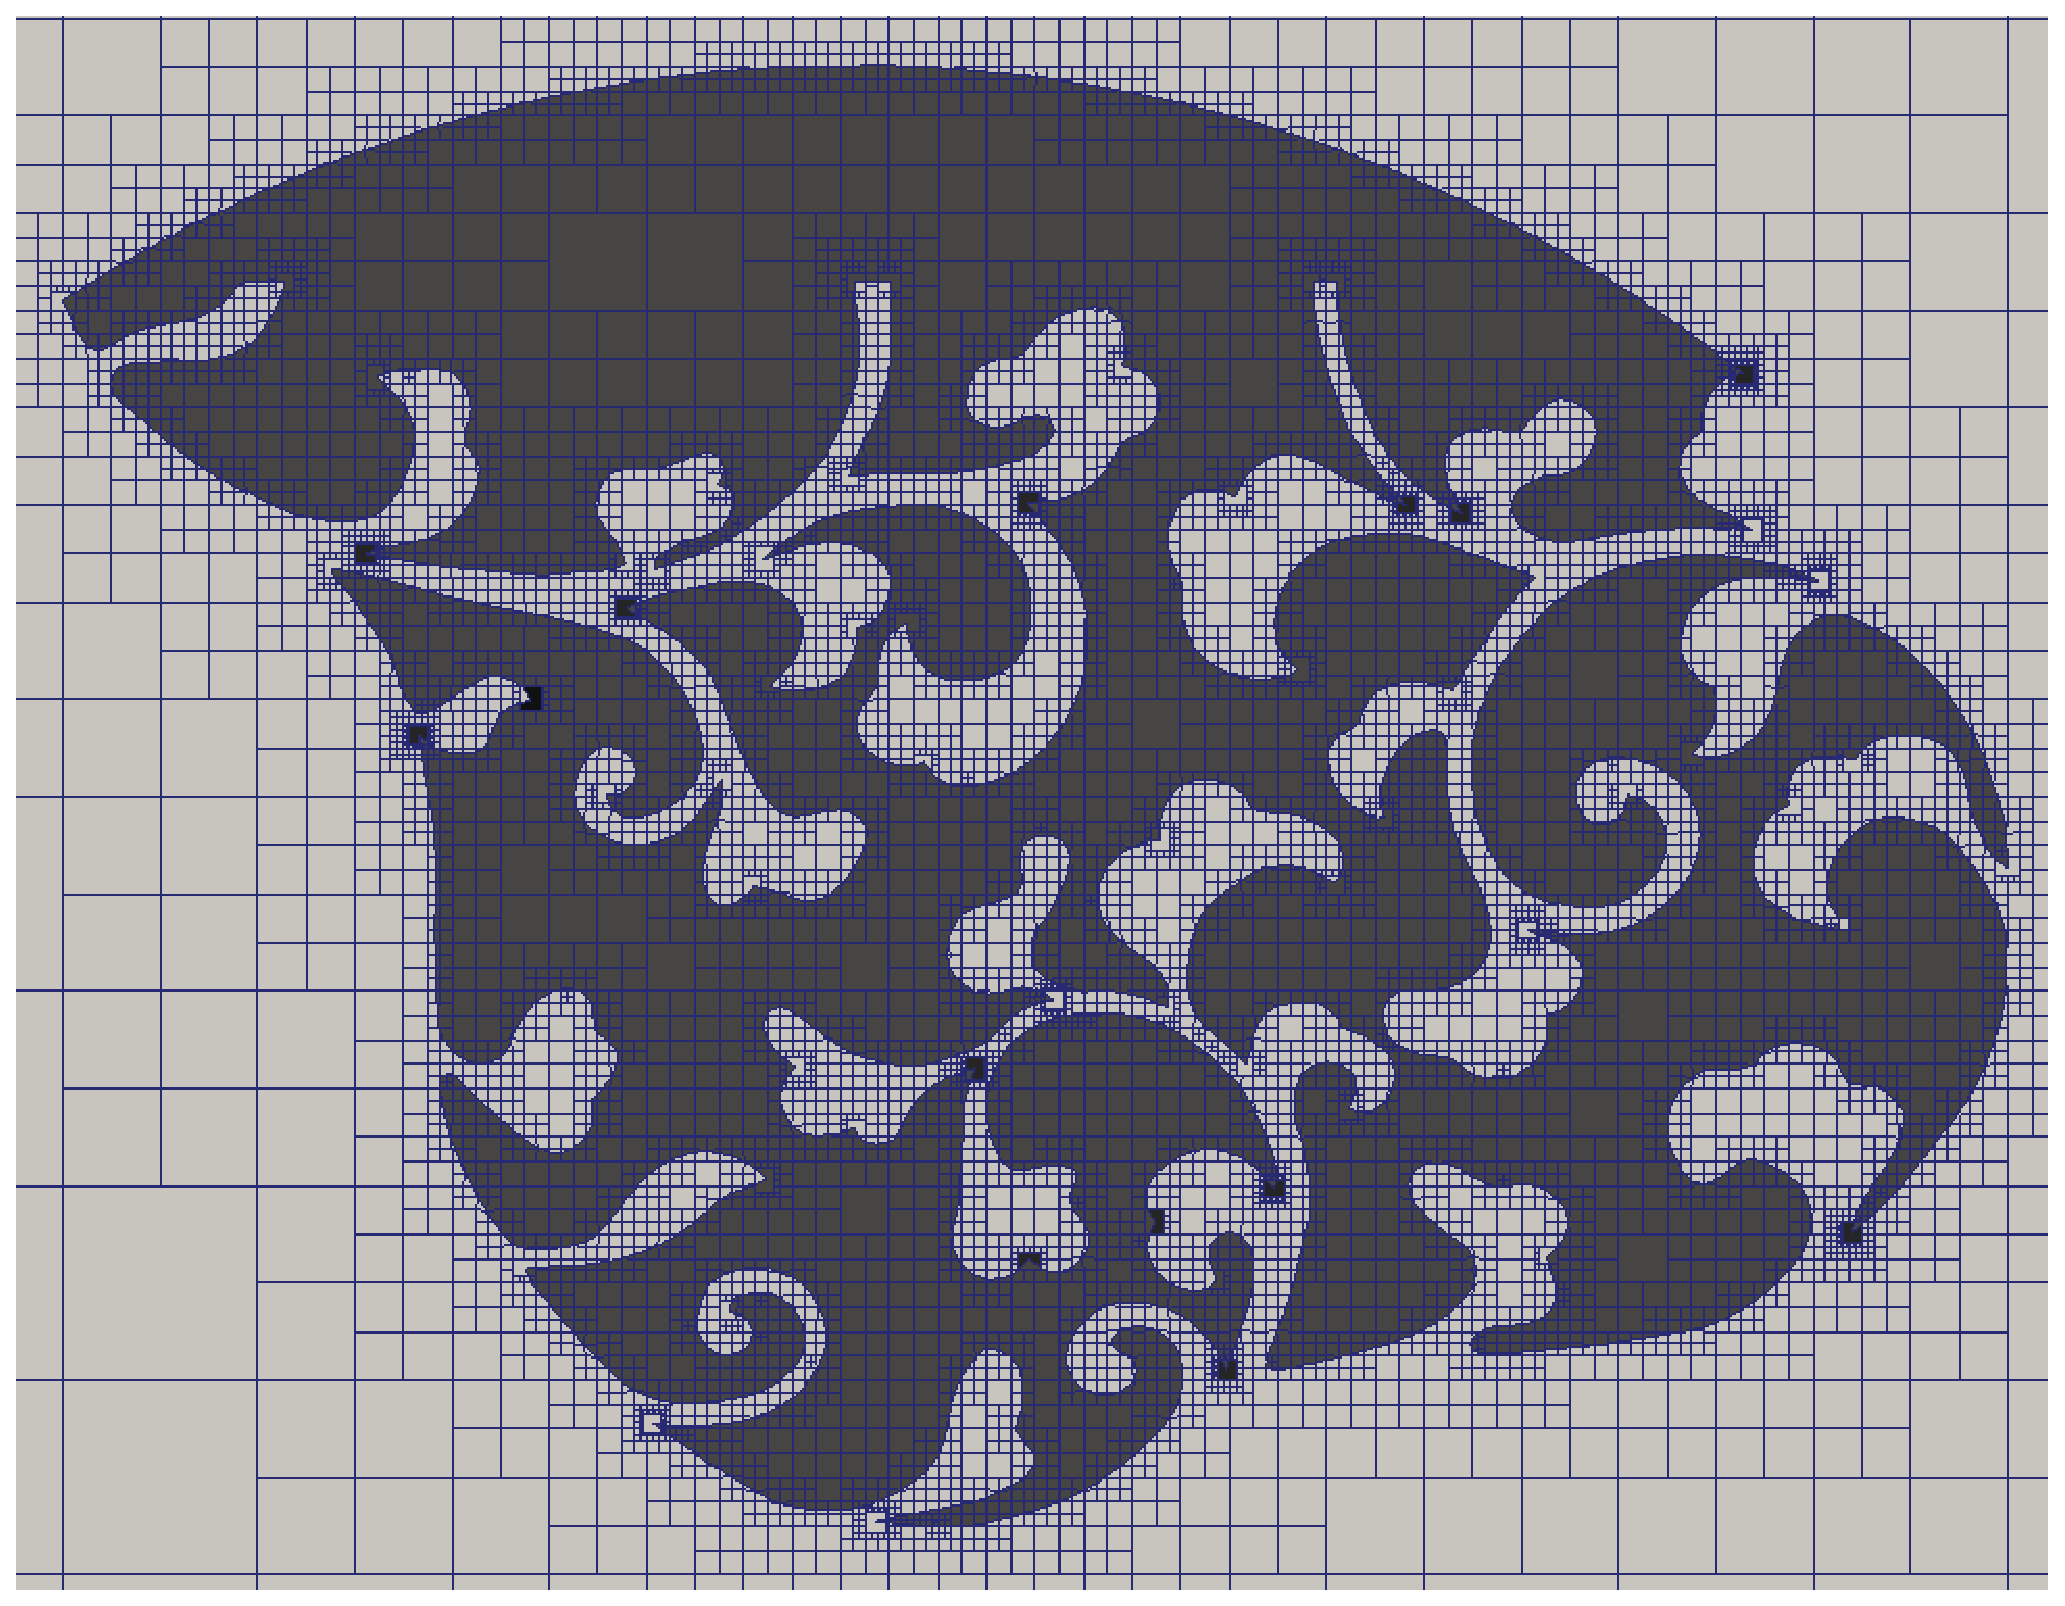
\includegraphics{quadtree/ex_images/qdt_ex_mesh_flower.eps}
        }
        \caption{Mesh for flowers}
    \end{subfigure}
    \\
    \begin{subfigure}[b]{1\linewidth}
        \centering
        \scalebox{0.3}{
            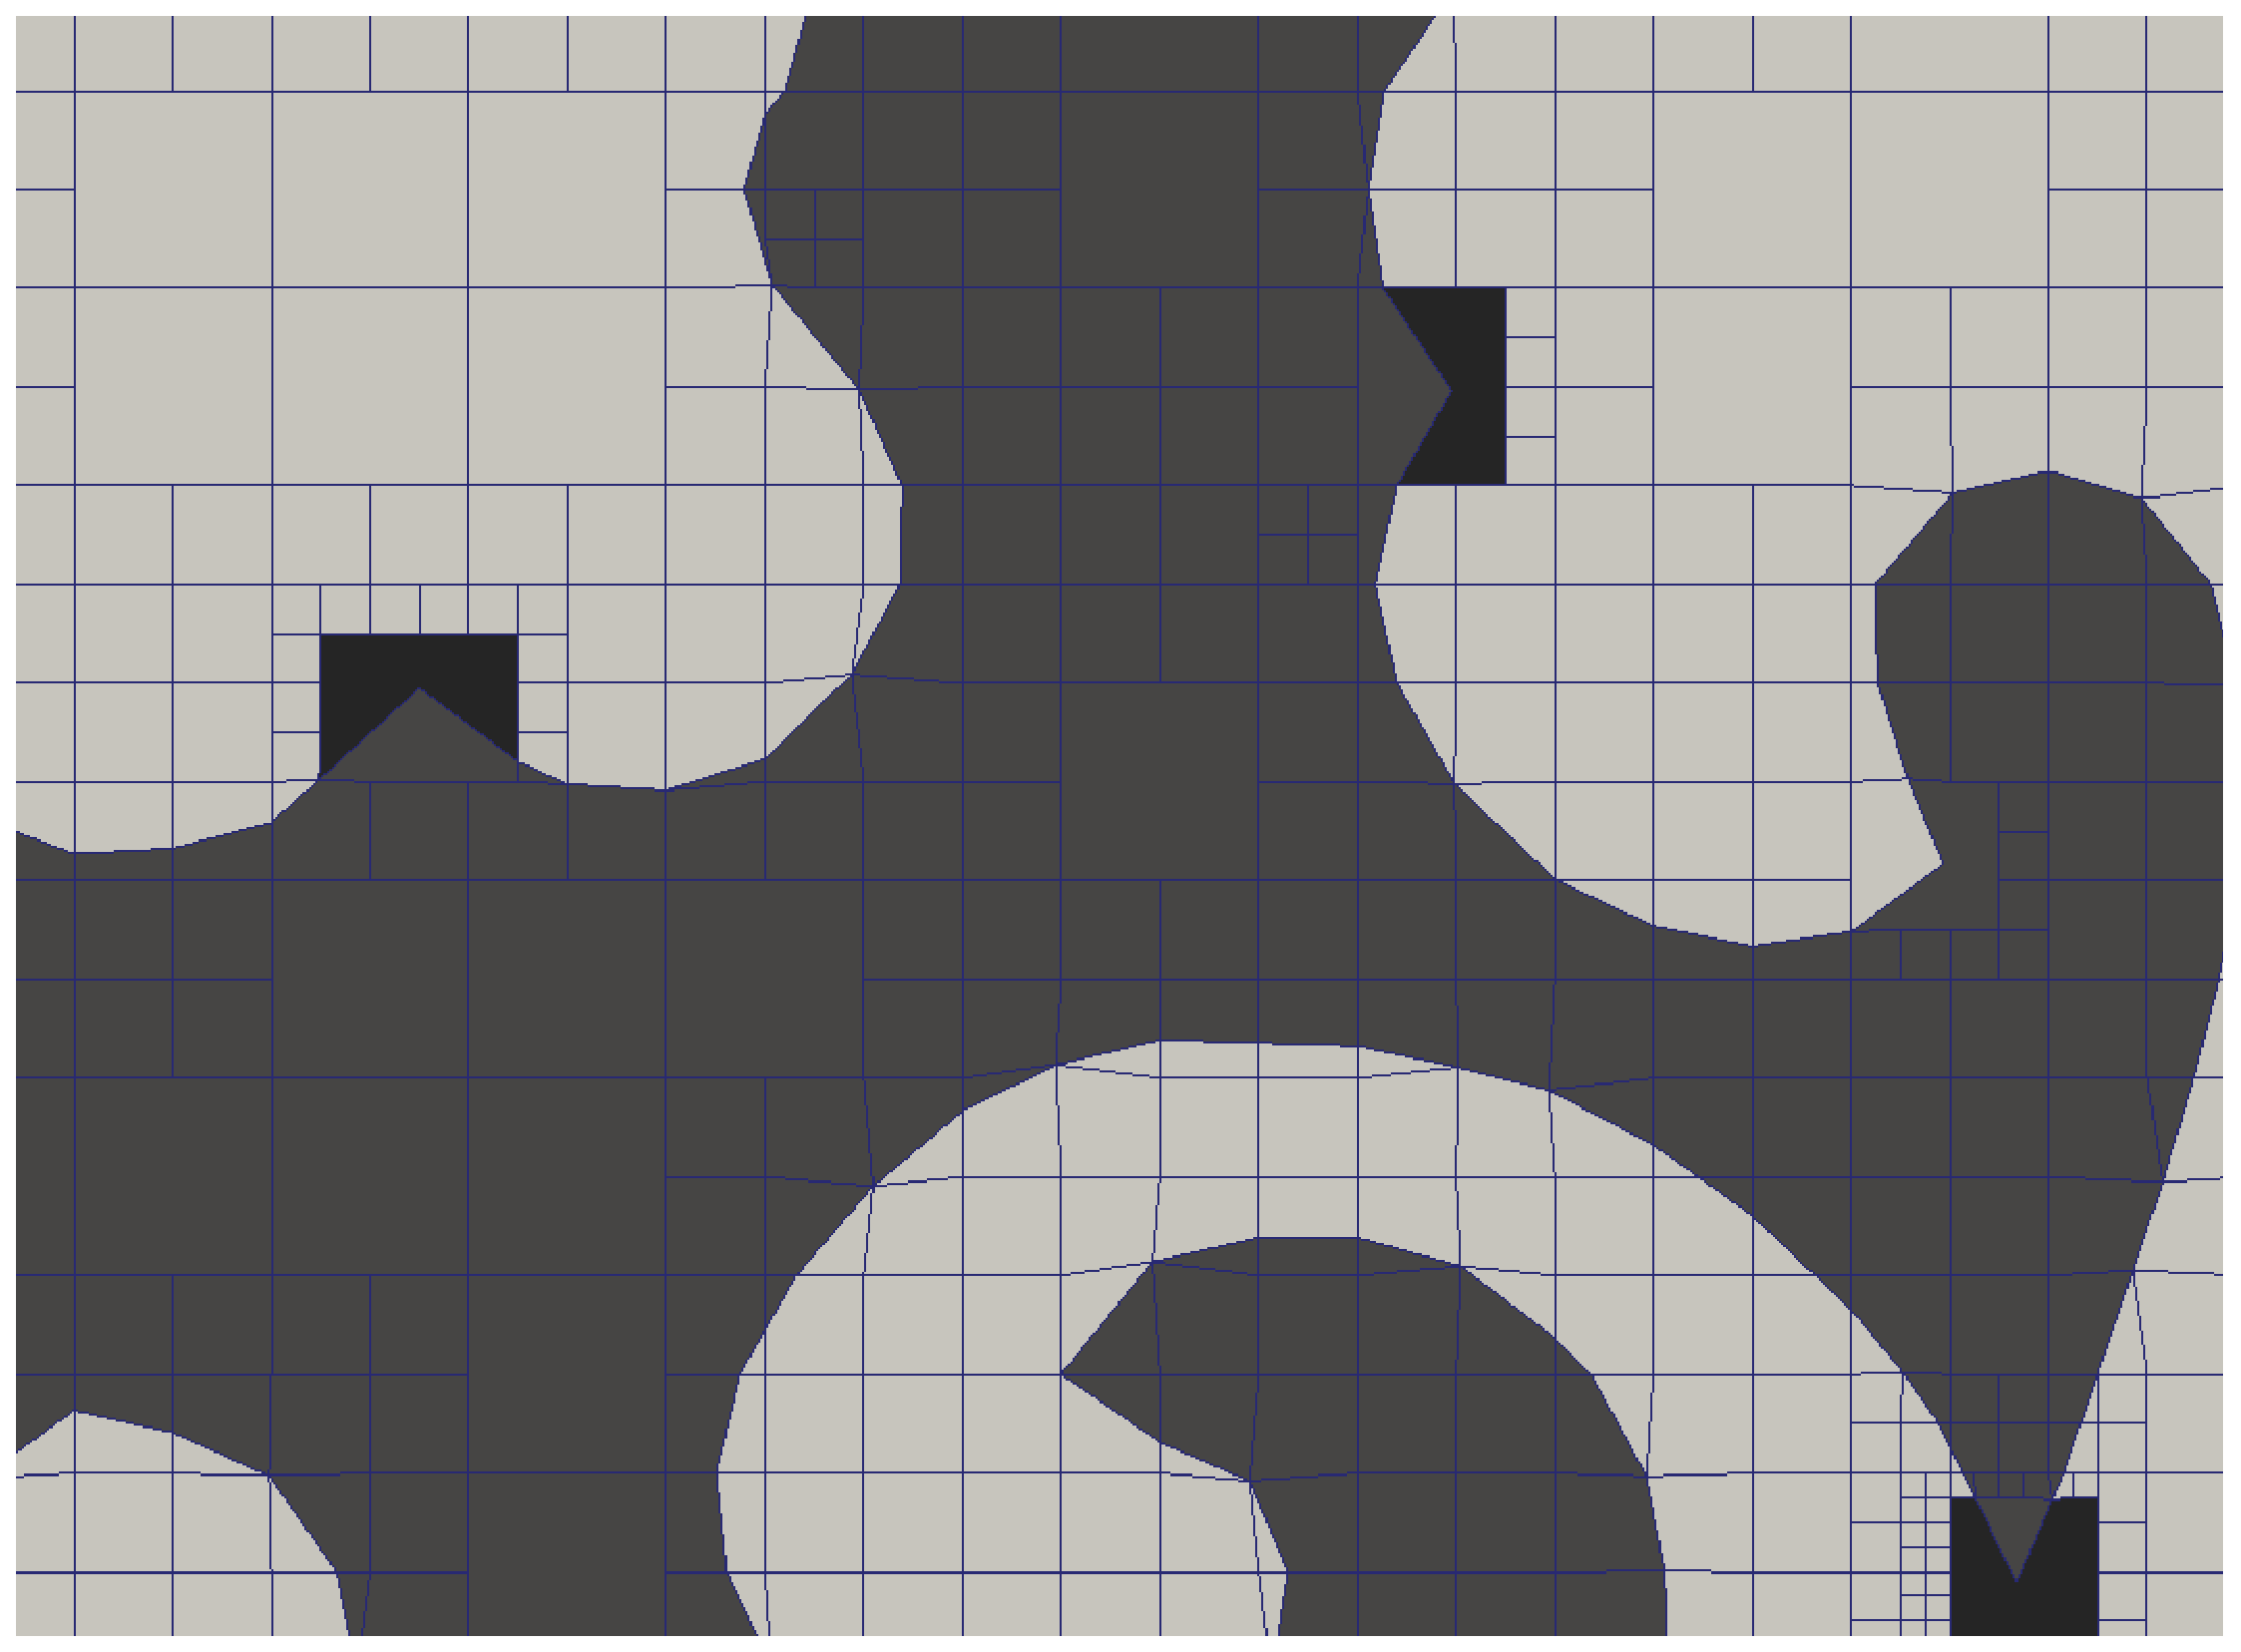
\includegraphics{quadtree/ex_images/qdt_ex_mesh_flower_sharp_corners.eps}
        }
        \caption{Mesh for flowers : Sharp corners treatment}
    \end{subfigure}
\end{figure}

\begin{figure}[h!]
    \begin{subfigure}[b]{1\linewidth}
        \centering
        \scalebox{0.3}{
            
\includegraphics{quadtree/ex_images/qdt_ex_mesh_wolli.eps}
        }
        \caption{Mesh for woolworth logo : Different colors for differnet materials}
    \end{subfigure}
    \\
    \begin{subfigure}[b]{1\linewidth}
        \centering
        \scalebox{0.3}{
            \includegraphics{quadtree/ex_images/qdt_ex_mesh_wolli_sharp_corner.eps}
        }
        \caption{Mesh for woolworth logo : Sharp conors treatment}
    \end{subfigure}
\end{figure}


\section{Conclusions}
In this chapter, we employed the IGES file directly from the CAD output to generate the quadtree mesh automatically.
The accuracy, effectiveness and the convergence properties of the proposed method are demonstrated with benchmark problems in linear elasticity mechanics.
From the numerical studies, it can be observed that the quadtree mesh yield better accuracy when compared to uniform mesh with same degree of freedoms.
The proposed methods provides a systematic and automatic mesh generation algorithm that can produce high quality mesh.
CAD design file can be used directly and the exact geometry can also be retained, which can largely reduce human efforts involved in numerical analysis.
Moreover, it can also help to reduce the analytical error as the difference in the geometric representation is minimized.
Computational efficiency can also be improved via utilizing the pattern of the quadtree.

